\documentclass[aspectratio=169]{beamer}
\usepackage[english]{babel}
\usepackage[T1]{fontenc}
\usepackage[utf8]{inputenc}
\usepackage{cite}
\usepackage{tikz}
\usetikzlibrary{shapes,arrows,fit,calc,positioning,automata}
\usepackage{eurosym}
\usepackage{caption}
\captionsetup[figure]{labelformat=empty}
\usepackage{microtype}



\title{{\normalsize Development and test of FPGA firmware extensions for the configuration and readout\\ of the ABACUS\_v2 chip for beam monitoring applications in hadron therapy}}
\author[Stefan Zugravel]{Candidate: \\ Stefan Cristi Zugravel \\ --------------------------------- \\ Supervisor: \\ Dott. Luca Pacher\\ ---------------------------------  \\ Co-Supervisor: \\ Prof. Vincenzo Monaco}
\date{\today}
\institute[UniTo]{University of Turin}
\logo{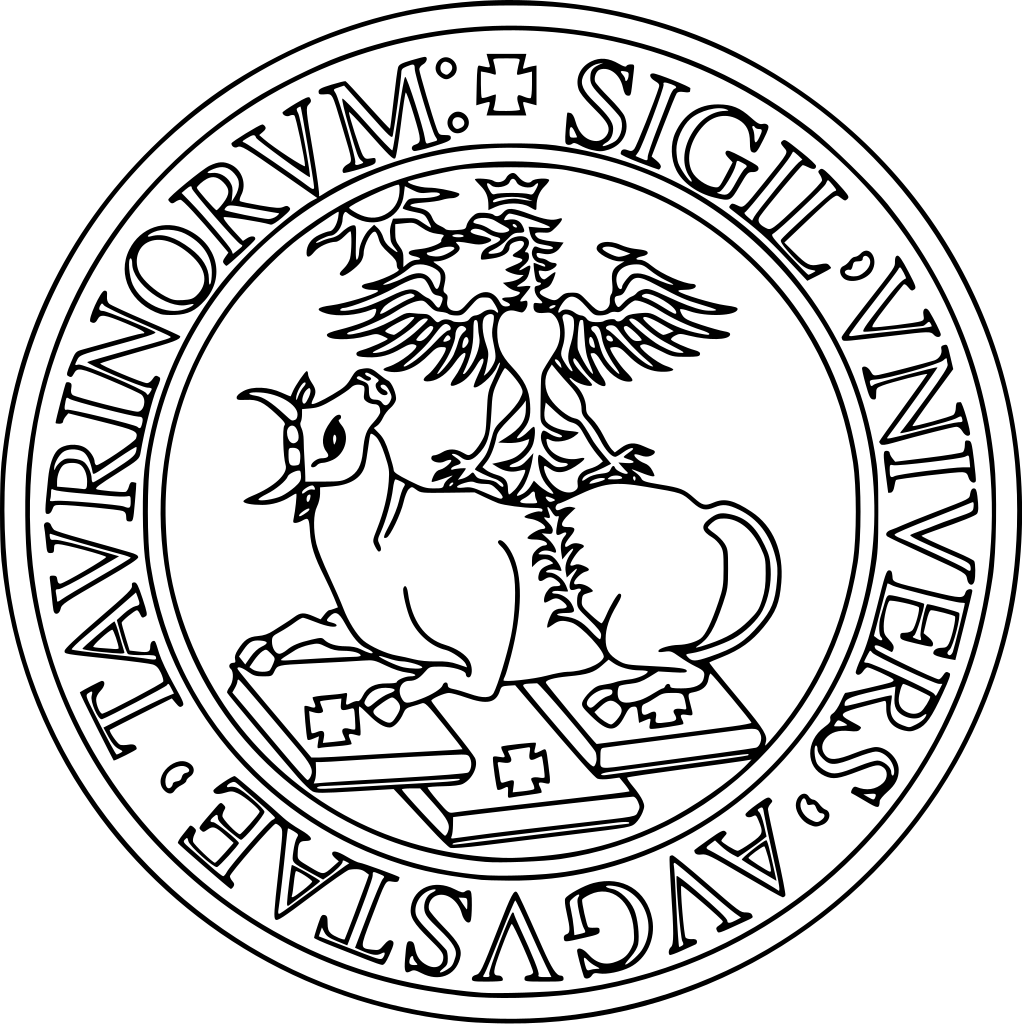
\includegraphics[width=10mm]{IMG/Unito.png}}
\usetheme{Madrid}
%\setbeamercovered{dynamic}
\setbeamertemplate{footline}[frame number]
\setbeamertemplate{navigation symbols}{}
\begin{document}
	
	\begin{frame}[noframenumbering]		
		\maketitle
	\end{frame}

	\begin{frame}[noframenumbering]
	\frametitle{Table of contents}
		\begin{columns}
			\hspace*{15mm}
			\column{0.3 \textwidth}
				\begin{center}
					\tableofcontents
				\end{center}
			\column{0.7 \textwidth}
				\begin{center}
					
\includegraphics[width=0.55 \textwidth]{IMG/LOGOINFN.PNG}
					
\includegraphics[width=0.55 \textwidth]{IMG/Move_IT_logo.PNG}
				\end{center}
		\end{columns}
	\end{frame}

%%%%%%%%%%%%%%%%%%%%%%%%%%%%%%%%%%%%%%%%%%%%%%%%%%%%%%%%%%%%%%%%%%%%%%%%%%%%%%%%%%%%%%%%
	\section{Hadron therapy}
	
	\begin{frame}[plain, noframenumbering]
	%\frametitle{Hadron therapy, sensor and ASICs}
	\begin{center}
		{\Huge \fontfamily{qtm}\selectfont \color{blue} \textbf{Hadron therapy, sensor and ASICs}}
	\end{center}
	\end{frame}
	
	\begin{frame}
	\frametitle{Hadron therapy}
		\begin{columns}
		\column{0.40 \textwidth}
		\begin{center}
			\textbf{Hadron therapy} uses heavy charged particles (p, ${}^{12}$C ions) to administer a lethal dose to the tumor target minimizing the energy deposited in the surrounding healthy tissues.
			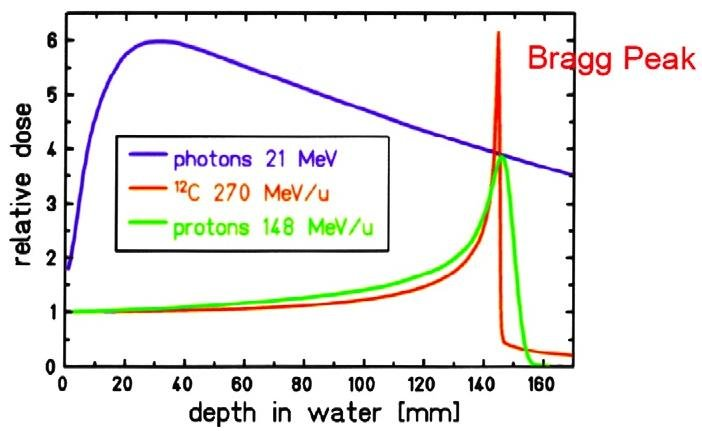
\includegraphics[width=0.95 \textwidth]{IMG/Bragg_Peak.PNG}
		\end{center}
		\column{0.60 \textwidth}
		
			{\color{blue} Advantages compared to x-ray radiotherapy:}
			\begin{itemize}
				\item Maximum dose delivered deep into tissue (Bragg peak that depends on the energy)
				\item Greater conformation of the dose to the tumor
				\item Conservation of the healthy tissues 
			\end{itemize}
		\vspace{1 cm}
			{\color{blue} Advanced treatment techniques use thin proton beams. \\ Typical parameters (TIFPA examples):}
			\begin{itemize}
				\item FWHM 3$\div$7 mm
				\item Beam rates $10^6\div10^{10}$ p/s
				%\item Current  1$\div$320 nA
				\item Energy  70$\div$228 MeV $\rightarrow$ (4$\div$32) cm in water
			\end{itemize}
		
		\end{columns}
	\end{frame}

	\begin{frame}
		\frametitle{Dose delivery system}
		\begin{columns}
			\column{0.5 \textwidth}
			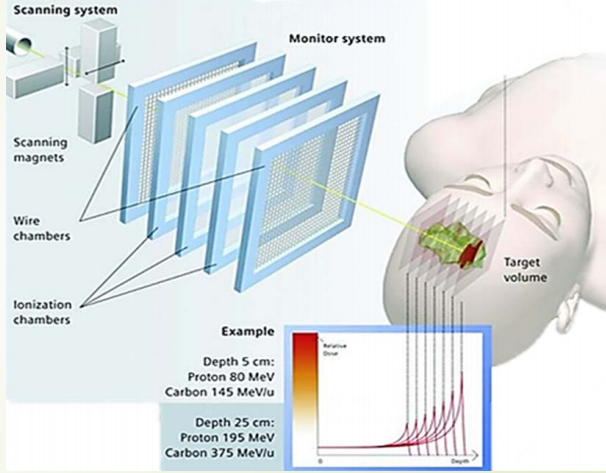
\includegraphics[width=0.95 \textwidth]{IMG/Beam_Monitoring.PNG}
			\column{0.5 \textwidth}
			{\color{blue} \textbf{Active spot scanning:}}
			\begin{itemize}
				\item Acquisition of morphological data by CT (\textbf{C}omputed \textbf{T}omography) and tumor volume identification
				\item Subdivision of the tumor into spots organized in layers of different depths corresponding to different beam energies
				\item Transverse scanning by deflecting the pencil beam via a pair of magnets
				\item Longitudinal scan by varying the energy of the beam
			\end{itemize}
		\end{columns}
	\vspace{0.5 cm}
	{\color{blue} Monitoring in real-time beam parameters (direction and \textbf{number of particles} delivered) \newline is extremely important in order to distribute the dose accurately}
	\end{frame}
	%I rivelatori controllano il trattamento, sulla base di queste informazioni viene controllata la posizione, la direzione e l'energia del fascio in tempo reale
	%Come si comportano dei rivelatori al silicio?

	\begin{frame}
		\frametitle{Beam monitoring}
		\begin{columns}
			\column{0.04 \textwidth}
			\column{0.2 \textwidth}
			\begin{center}
				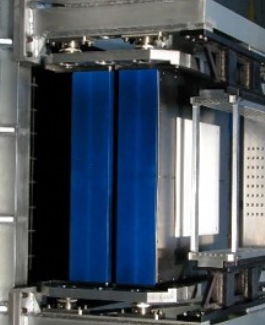
\includegraphics[width=0.95 \textwidth]{IMG/Ionization_Chamber.PNG}
			\end{center}
			\begin{center}
				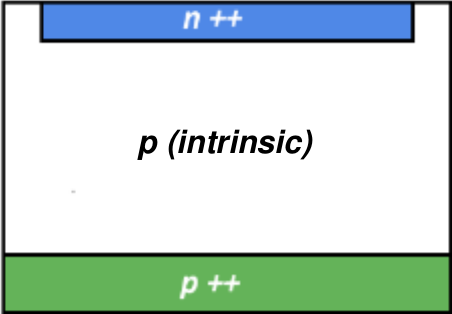
\includegraphics[width=0.95 \textwidth]{IMG/Solid_State_Detector.PNG}
			\end{center}
			\column{0.38 \textwidth}
			{\color{blue} Ionization chambers}
			\newline
			\textbf{Advantages}
			\begin{itemize}
				\item Structural integrity
				\item Radiation resistance
			\end{itemize}
			\textbf{Disadvantages}
			\begin{itemize}
				\item Slow response times $\approx 100\:\mu s$
				\item Limited sensitivity (>$10^4$ p)
				\item Indirect measurement of the number of particles  (mandatory to know the beam energy)
			\end{itemize}
			\column{0.38 \textwidth}
			{\color{blue} Solid state detectors}
			\newline
			\textbf{Advantages}
			\begin{itemize}
				\item Fast response times $\approx 1-2$ ns
				\item Ideally, sensitive to the single particle
				\item High spatial-temporal resolution
			\end{itemize}
			\textbf{Disadvantages}
			\begin{itemize}
				\item Complex and fast readout electronics
				\item Damage from radiation
				\item pile-up effects at high\newline rates
			\end{itemize}
		\end{columns}
	\end{frame}


	
	\begin{frame}
	\frametitle{UFSD/LGAD sensors}
	\begin{columns}
	\column{0.35 \textwidth}
		\begin{center}	
			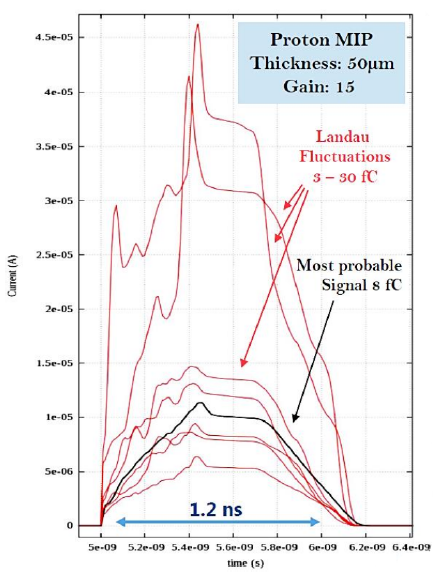
\includegraphics[width=0.9 \textwidth]{IMG/LGAD_Signal.PNG}
		\end{center}
	\column{0.65 \textwidth}
	\begin{columns}
		\column{0.4 \textwidth}
			\begin{center}
				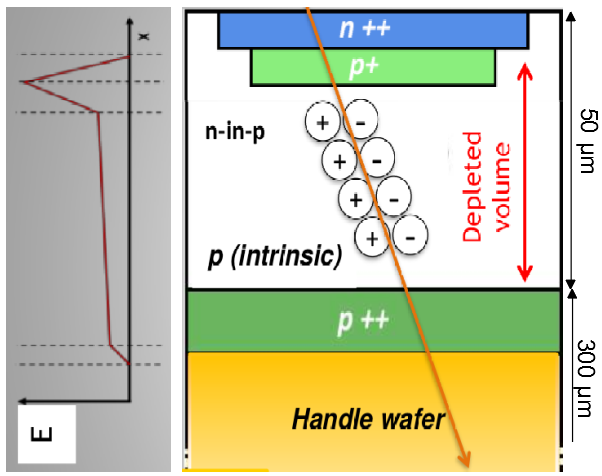
\includegraphics[width=1 \textwidth]{IMG/UFSDLGAD.PNG}
			\end{center}
		\column{0.6 \textwidth}
		\begin{center}
			We need \textbf{thin} detectors to have \textbf{short} signals (pile-up reduction), but thin detectors also have low \textbf{SNR}
		\end{center}
	\end{columns}
		\begin{itemize}
			\item \textbf{U}ltra \textbf{F}ast \textbf{S}ilicon \textbf{D}etector/\textbf{L}ow \textbf{G}ain \textbf{A}valanche \textbf{D}iode
			\item Charge multiplication in $p^+ / n^{++}$ junction 
			\item 50$\mu$m sensor thickness (active region)
			\item Internal gain of \textbf{10-15} 
			\item Trapezoidal signal of $\approx$\textbf{1.5ns}\newline
				{\color{blue} Capable of detecting single particle }
			\item LGAD allows to increase SNR 
		\end{itemize}
	\end{columns}
	\end{frame}
	%mettere figura delle strip che usiamo noi
	%Per spessori piccoli il segnale è piccolo
	%Abbiamo bisogno di sensori piccoli perché la frequenza massima a cui possiamo contare dipende dalla durata del segnale
	%Servono spessori piccoli per avere segnali veloci 
	%Idealmente dovremmo usare i pixel
	%LGAD mi permette di aumentare il rapporto segnale-su-rumore
	%Aggiungere segnale dell'LGAD

	\section{Move\_IT}
	
	\begin{frame}
	\frametitle{MoVe\_IT INFN project}
	\begin{center}
		{\Large \color{blue} MoVe\_IT = \textbf{Mo}deling and \textbf{Ve}rification for \textbf{I}on beam \textbf{T}reatment planning }
		\newline
		Prove the ability of \textbf{LGAD} detectors to discriminate individual protons and to count their number up to fluxes of \textbf{100} MHz/cm$^2$ with an uncertainty of {\color{blue}less than \textbf{1}\%}, (\underline{clinical tolerance required})
	\end{center}
	\begin{columns}
		\column{0.6 \textwidth}
		\begin{itemize}
			\item Single proton counting
			\item Custom detector built ad hoc
			\item Area \textbf{3x3} cm${}^2$ with \textbf{144} Strips
			\item Max proton flux= $10^8$ $\frac{p}{s \cdot cm^2}$ ({\color{blue} Error < \textbf{1}\%})
			\item 50$\mu$m sensor thickness (active region)
			\item Two orthogonal directions
		\end{itemize}
		\column{0.4 \textwidth}
		\begin{center}
			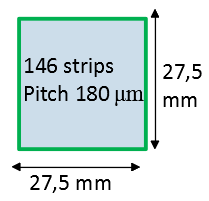
\includegraphics[width=0.7 \textwidth]{IMG/Detector.PNG}
		\end{center}
	\end{columns}
	\end{frame}

	\begin{frame}
	\frametitle{ABACUS\_v2 ({\small \textbf{A}synchronous-logic-\textbf{B}ased \textbf{A}nalog \textbf{C}ounter for \textbf{U}ltra fast \textbf{S}ilicon strips}) }
	\vspace*{-2mm}
	\begin{columns}
		\column{0.2 \textwidth}
		\begin{center}
				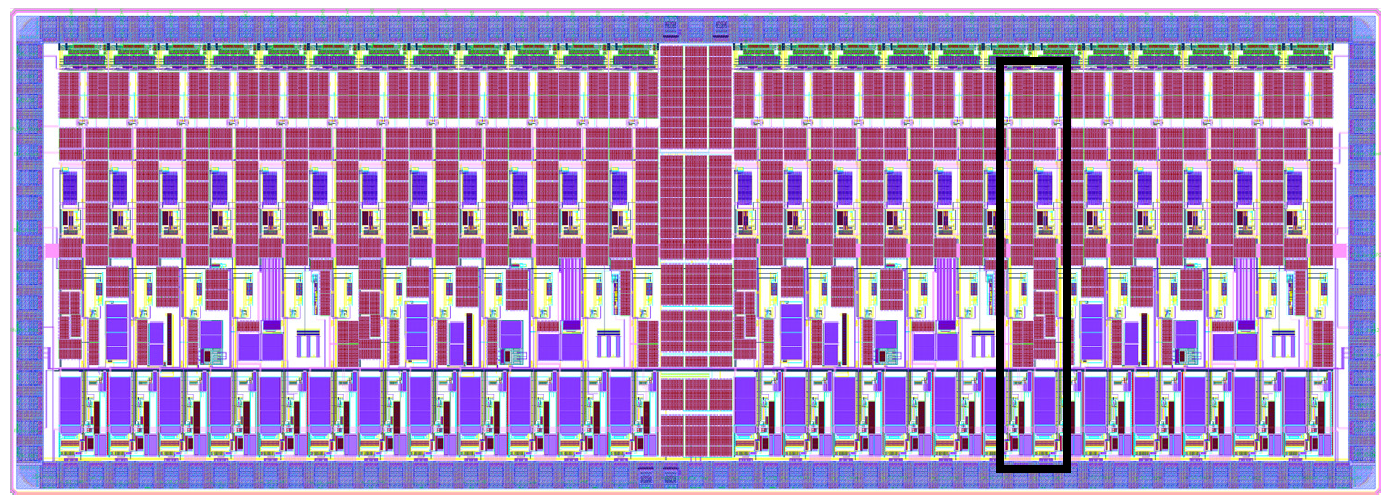
\includegraphics[width=2.45 \textwidth, angle=90]{IMG/ABACUS2.png}
		\end{center}
		\column{0.8 \textwidth}
		%\begin{center}
		%	{\color{blue} \textbf{ABACUS\_v2}}
		%\end{center}
		\begin{columns}
			\column{0.5 \textwidth}
			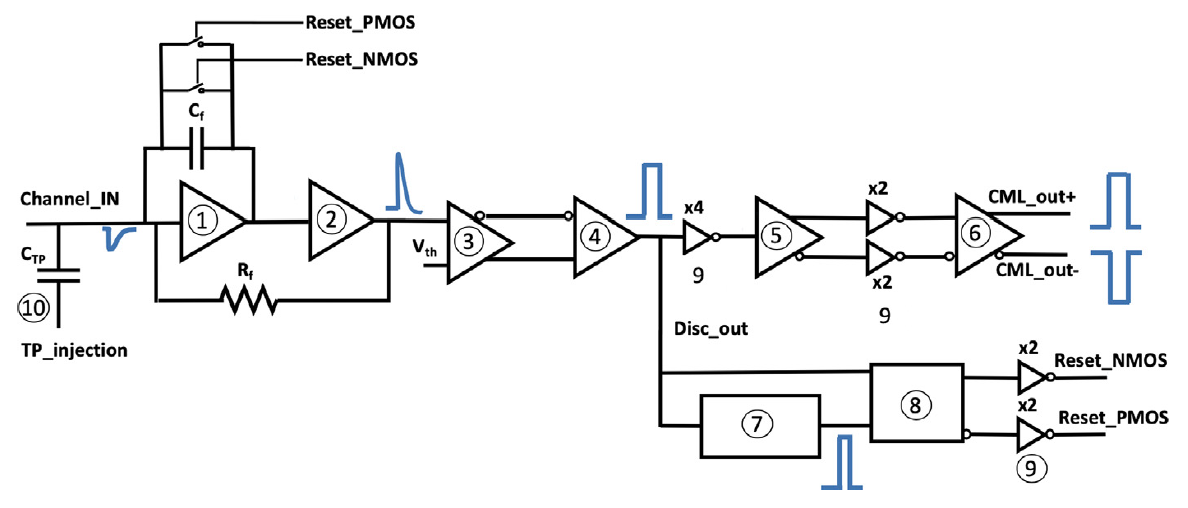
\includegraphics[width=0.99 \textwidth]{IMG/ABACUS_channel.PNG}
			{\color{blue} Channel structure }
			{\footnotesize 
			\begin{itemize}
				\item Low noise \textbf{Charge} Sensitive Amplifier (\textbf{CSA})
				\item Fast discriminator for \textbf{binary} readout
				\item Discriminator driven by \textbf{2 DACs}
				\begin{itemize}
					%the discriminator threshold is setted with an external value and, in order to uniform the channels an internal DAC is used.
					{\footnotesize
					\item[$-$] External 16b DAC $\rightarrow$ global Vth
					\item[$-$] Internal 6b DAC $\rightarrow$ Th tuning
				}
				\end{itemize}
				\item \textbf{CML} converter (propagate signal)
				\item \textbf{Fast} reset signal (reduce dead time)
			\end{itemize} }
			\column{0.5 \textwidth}
			{\color{blue} Chip specifications }
			\begin{itemize}
				\item Die size \textbf{4.95 }x \textbf{1.935} mm$^2$
				\item \textbf{110} nm CMOS technology
				\item \textbf{24} channels
				\item \textbf{I2C} controller for digital configuration
				\item Max frequency >\textbf{100} MHz
				\item Input charge \textbf{3-140} fC
				\item Dead time <\textbf{10}ns
				\item SNR>\textbf{10}
				\item Full digital I/O interfaced \\ with \textbf{FPGA}
			\end{itemize}
		\end{columns}
		%%%
		%\begin{itemize}
		%	\item \textbf{Fast} reset signal (reduce dead time)
		%\end{itemize}
		%%%
	\end{columns}
	\end{frame}

		

		\begin{frame}
	\frametitle{FPGA  (\textbf{F}ield \textbf{P}rogrammable \textbf{G}ate \textbf{A}rray)}
	\begin{columns}
		\column{0.5 \textwidth}
		\begin{center}
			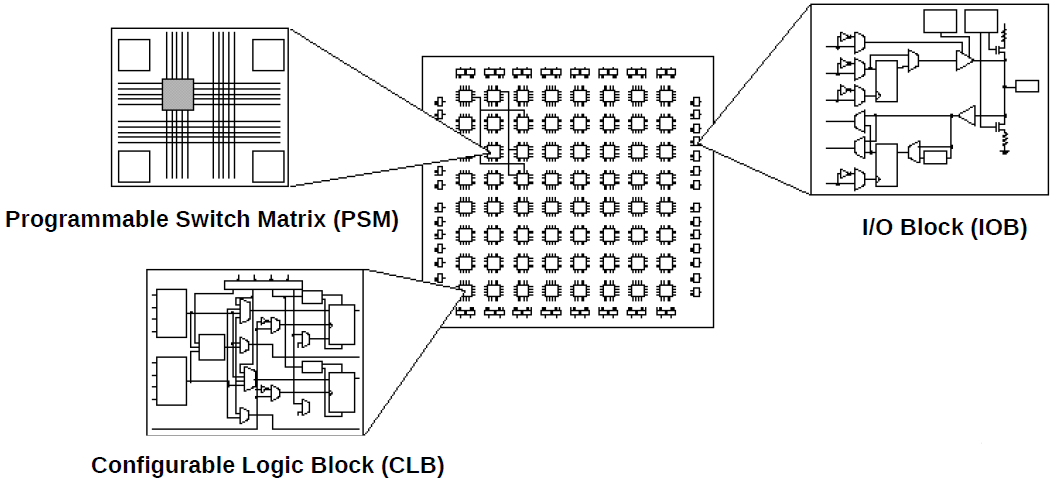
\includegraphics[width=0.7 \textwidth]{IMG/FPGA_PARTS}
		\end{center}
		\column{0.5 \textwidth}
		\begin{center}
			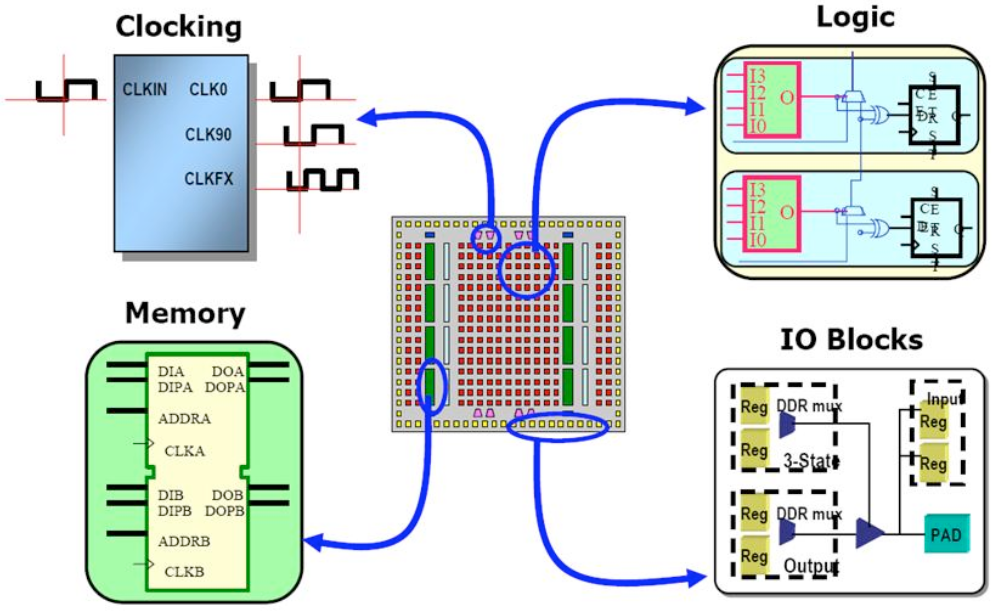
\includegraphics[width=0.6 \textwidth]{IMG/FPGA2}
		\end{center}
	\end{columns}
		\vspace{2mm}
		\begin{itemize}
			\item A FPGA is a digital integrated circuit that can be programmed to implement any digital~functionality after manufacturing – hence the term \textbf{field-programmable}
			\item In principle, \textbf{programmable infinite times} with no limitations
			\item \textbf{High flexibility}: it can be implemented \textbf{any digital function}
			\item \textbf{Fast} and \textbf{cheap} prototyping: \textbf{out of the box} solution: no layout or masks
			%\item {\color{orange} Power hungry, slow compared to \textbf{ASICs} and expensive on large-scales}
			\item \textbf{HDL} (\textbf{H}ardware \textbf{D}escription \textbf{L}anguage) such as Verilog or VHDL are used to implement~and simulate the desired digital circuit
		\end{itemize}
	\end{frame}

\begin{frame}
	\frametitle{FPGA main tasks}
	\vspace*{-2.7mm}
	\begin{center}
		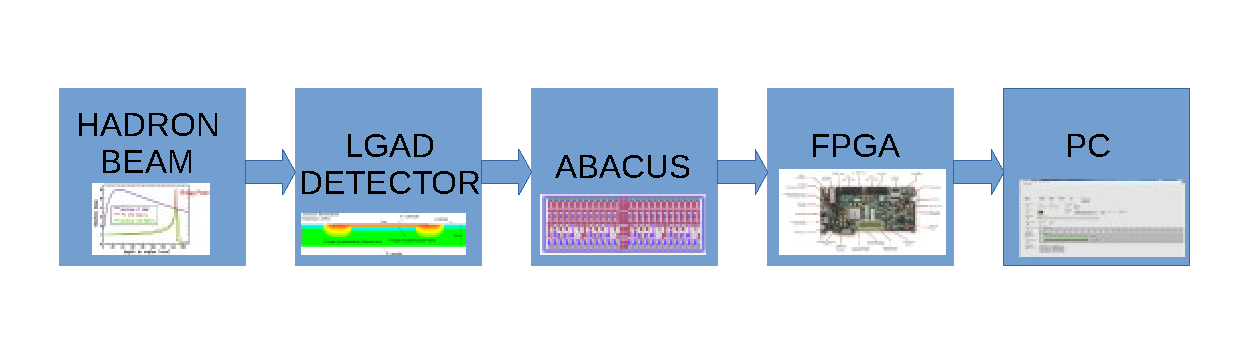
\includegraphics[width=0.85 \textwidth]{IMG/Block_Diagram.pdf}
	\end{center}
	\vspace*{-5mm}
	\begin{center}
		{\Large \color{blue} What does the \textbf{FPGA} board do?}\\[3mm]
		\begin{itemize}
			\item Receives the \textbf{outputs} from the ABACUS chip
			\item For each channel counts the \textbf{number of pulses} (thus the number of particles) and the pulse duration
			\item For two adjacent channels counts the number of coincidence \textbf{AND} and \textbf{OR} (for pile-up correction)
			\item Sends the data to a \textbf{PC} via \textbf{Ethernet}/\textbf{UDP} protocol
			\item Configuration of \textbf{internal} and \textbf{external} DACs
		\end{itemize}
	\end{center}
\end{frame}

	
%%%%%%%%%%%%%%%%%%%%%%%%%%%%%%%%%%%%%%%%%%%%%%%%%%%%%%%%%%%%%%%%%%%%%%%%%%%%%%%%%%%%%%%%
\section{Experimental setup}

\begin{frame}[plain, noframenumbering]
\begin{center}
	{\Huge \fontfamily{qtm}\selectfont \color{blue} \textbf{Experimental setup}}
\end{center}
\end{frame}



	\begin{frame}
	\frametitle{Test boards}
		\begin{columns}
			\column{0.5 \textwidth}
			\begin{center}
				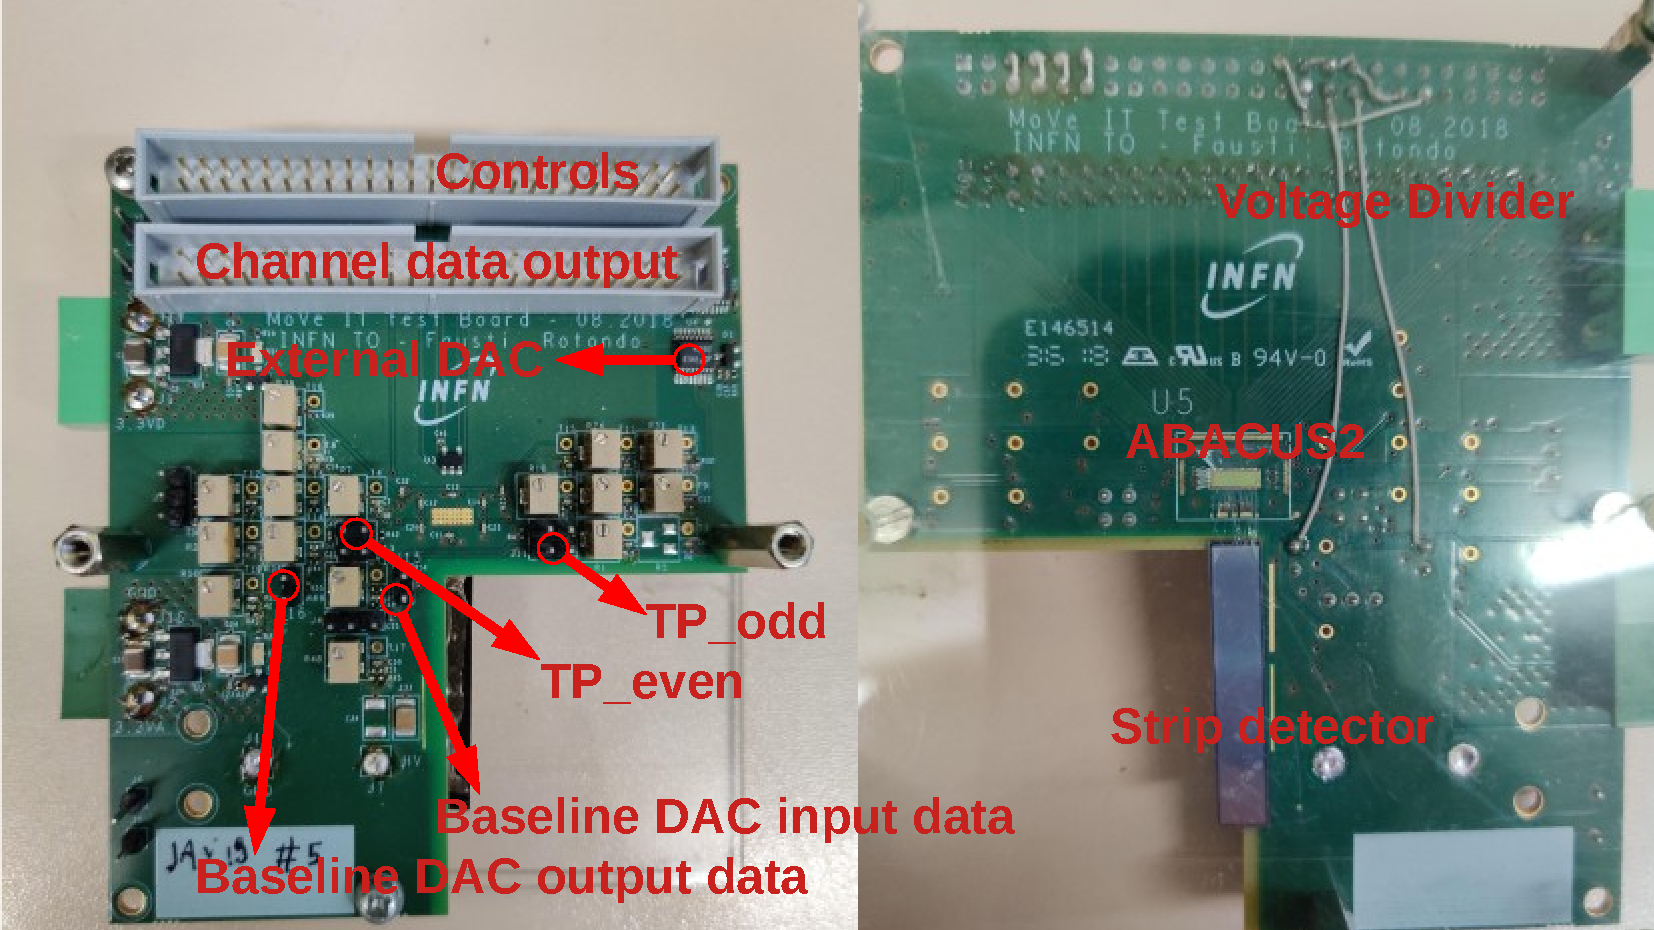
\includegraphics[width=0.99 \textwidth]{IMG/TestBoard.pdf}
			\end{center}
		{\hspace*{1.5cm}
		{\color{blue}ESA-ABACUS read-out board}
		\begin{itemize}
			\item \textbf{6 ABACUS} chips
			\item Able to read \textbf{144} strips
			\item \textbf{3} FPGA (Kintex7 KC705) needed
		\end{itemize}
			}
			\vspace*{1cm}
			\column{0.5 \textwidth}
			\hspace*{1.5cm}
			{\color{blue}ABACUS\_v2 test board}
			\begin{itemize}
				\item 1 \textbf{ABACUS} ASIC chip
				\item \textbf{CML} output to \textbf{FPGA}
				\item \textbf{I2C} input to internal DACs
				\item Possibility to \textbf{simulate} signals sending test pulses (TP) to even or odd channels
			\end{itemize}
		\begin{center}
			\vspace*{0.5cm}
			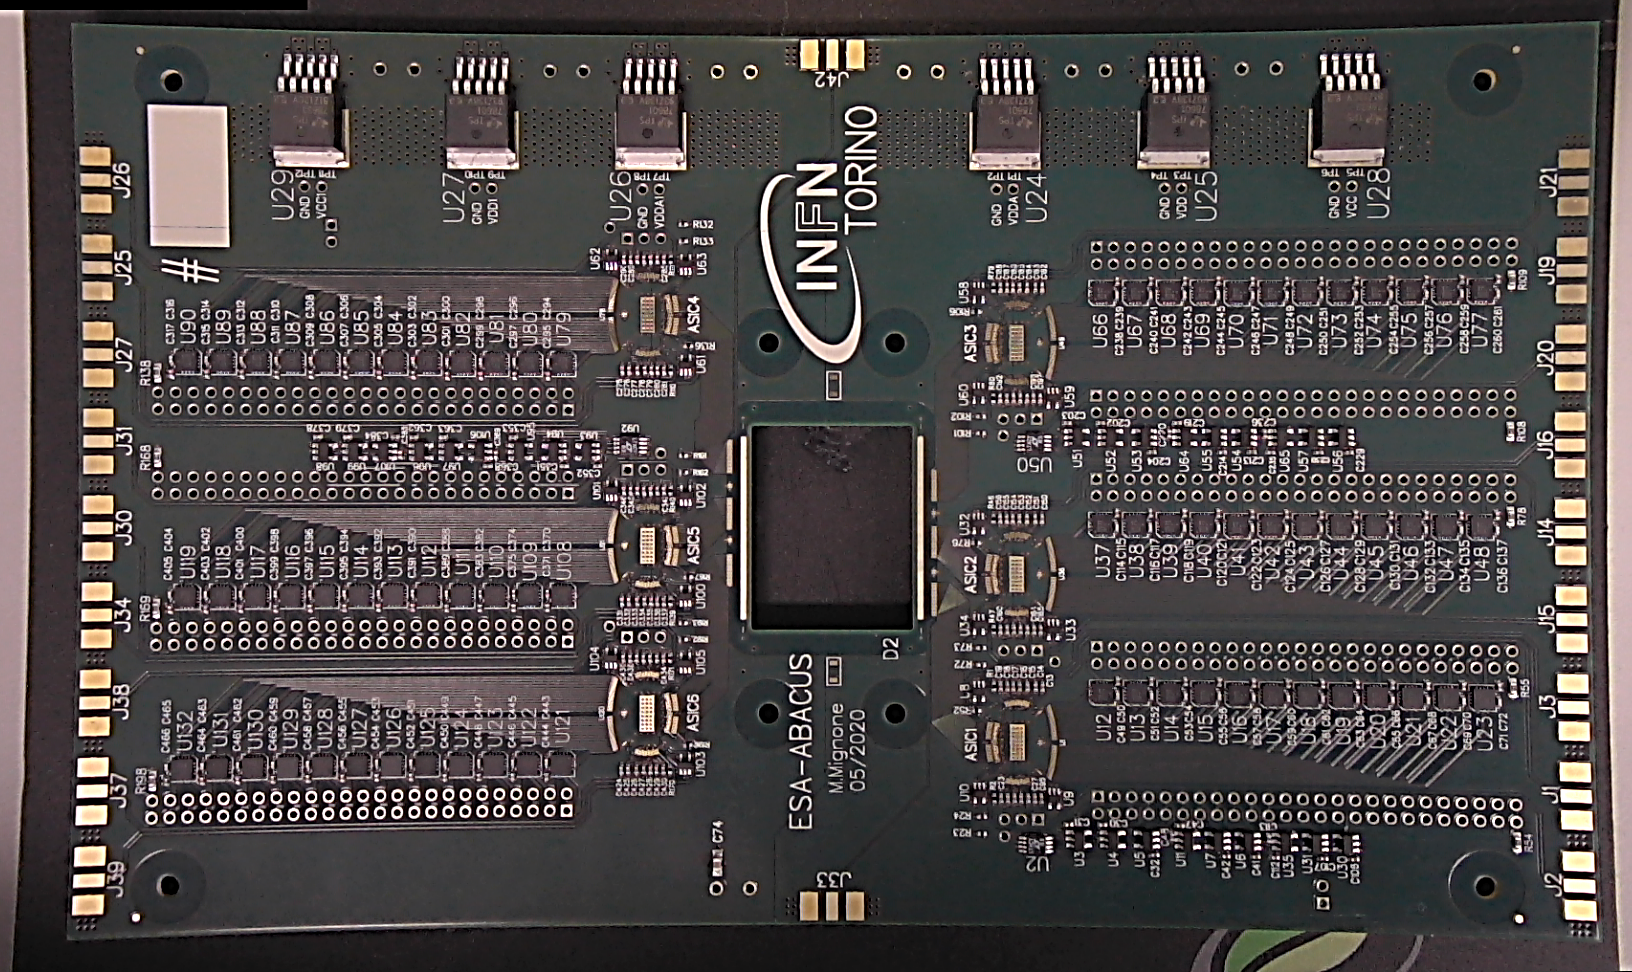
\includegraphics[width=0.6 \textwidth]{IMG/EsaAbacus.png}
		\end{center}
	
		\end{columns}	
	\end{frame}

	\begin{frame}
	\frametitle{Experimental setup}
		\begin{columns}
			\column{0.65 \textwidth}
			\begin{center}
				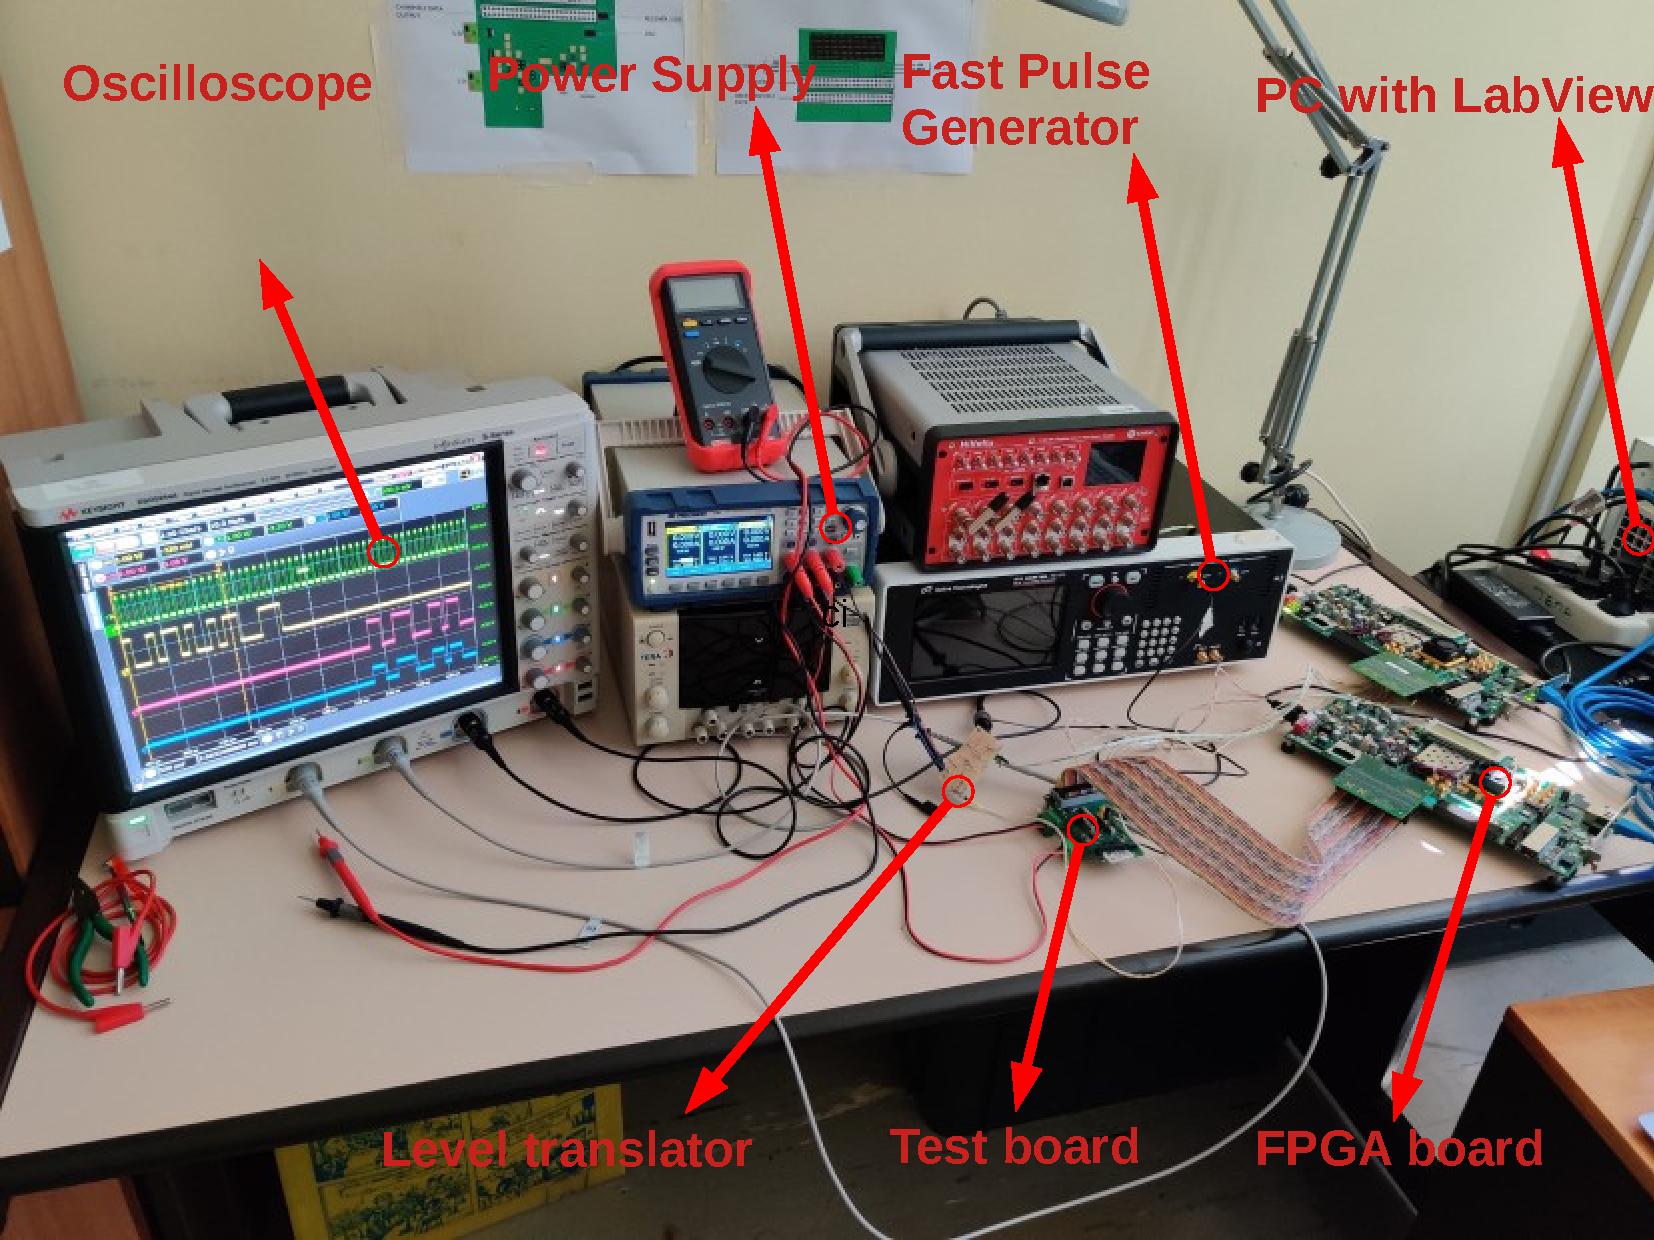
\includegraphics[width=0.95 \textwidth]{IMG/TestBench.pdf}
			\end{center}
			\column{0.35 \textwidth}
			\begin{itemize}
				\item Fast Pulse Generator
				\item Oscilloscope
				\item Power Supply
				\item Xilinx Kintex7 FPGA
				\item Test Board
				\item PC with LabView
				\item Level translator
			\end{itemize}
		\end{columns}
		
	\end{frame}


%%%%%%%%%%%%%%%%%%%%%%%%%%%%%%%%%%%%%%%%%%%%%%%%%%%%%%%%%%%%%%%%%%%%%%%%%%%%%%%%%%%%%%%%

	\section{Personal Contribution}
	
	\begin{frame}[plain, noframenumbering]
		\begin{center}
			{\Huge \fontfamily{qtm}\selectfont \color{blue} \textbf{Personal contribution to the project}}
		\end{center}
	\end{frame}
	
	
	\begin{frame}
	\frametitle{Personal Contribution}
	\begin{itemize}
		\item {\color{teal} Creation of a \textbf{debug} tool for the FMC connectors}
		\item {\color{teal} Creation of the level translation device for communication with the \textbf{FPGA}}
		\item {\color{teal} Firmware implementation of the read/write logic for internal DACs configuration \\ in the \textbf{ABACUS2} chip}
		\item {\color{teal} Addition of a \textbf{latch} in order to save into a \textbf{register} the current state of every counter}
		\item {\color{teal} Addition of a \textbf{timestamp} in order to obtain a more accurate rate calculation}
		%\item {\color{red} Addition of a configurable \textbf{mask} to calculate via firmware the \textbf{sum} of only certain selected channels}
	\end{itemize}
	\end{frame}
	
	\begin{frame}
		\frametitle{Firmware Debug Tool for FMC connector}
		%\small
		\begin{columns}
			\column{0.65 \textwidth}
			\begin{center}
				{\color{blue} XILINX KINTEX7 KC705}
				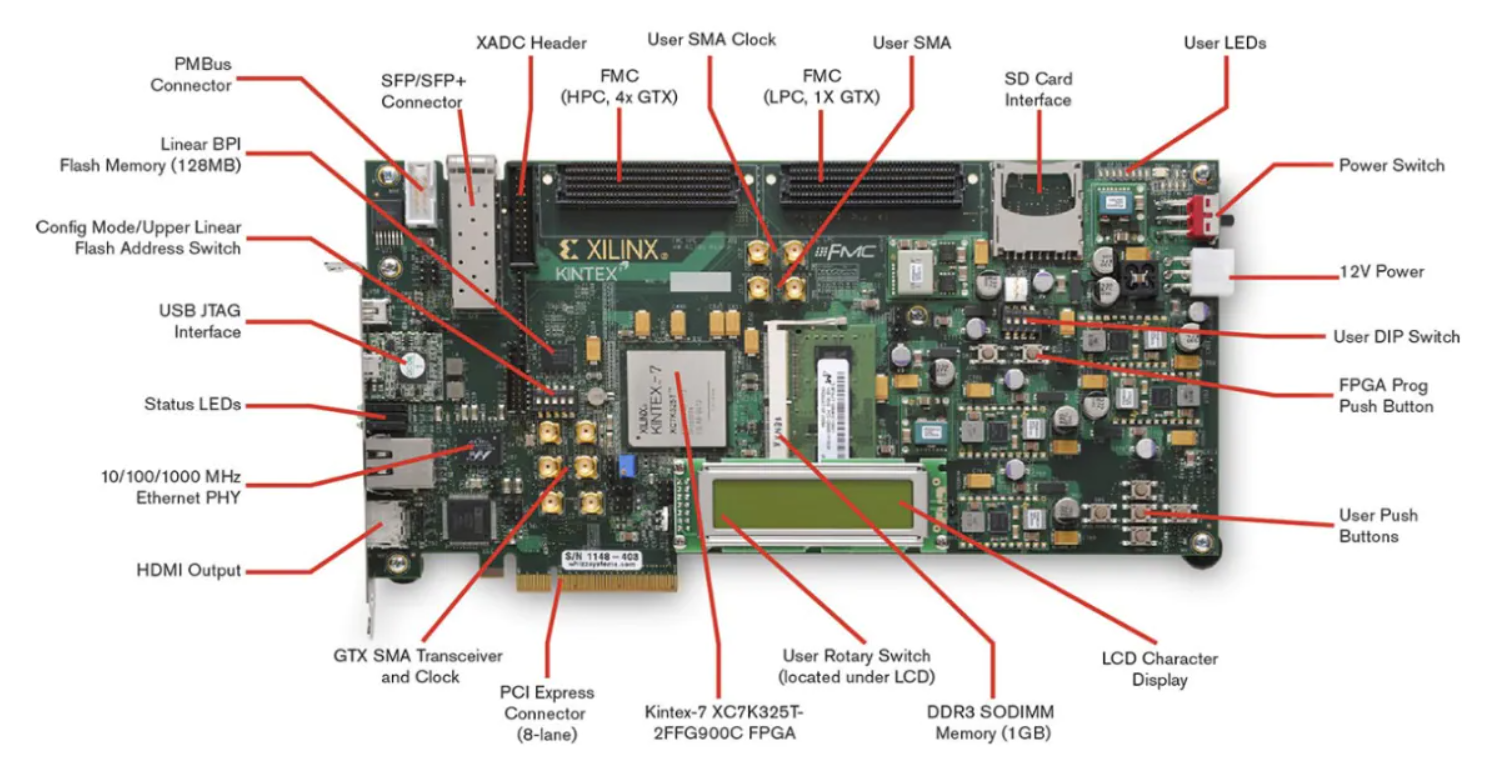
\includegraphics[width=1.0 \textwidth]{IMG/KC705.PNG}
			\end{center}
			\column{0.35 \textwidth}
			\textbf{FMC}{\tiny (\textbf{F}PGA \textbf{M}ezzanine \textbf{C}ard)} connector
			\begin{itemize}
				\item \textbf{LPC}= \textbf{L}ow \textbf{P}in \textbf{C}ount
				\item \textbf{HPC}= \textbf{H}igh \textbf{P}in \textbf{C}ount
				\item \textbf{LVDS} output 
			\end{itemize}
			\textbf{Debug}
			\begin{itemize}
				\item Set every pin as an \textbf{output}
				\item Switch state (0/1) with a DIP switch
				\item Measure voltages with multimeter
				\item Levels: high $\approx$ \textbf{1.5} V \\ low $\approx$ \textbf{0.7} V (\textbf{LVDS})
			\end{itemize}
		\end{columns}
	\end{frame}

	\begin{frame}
	\frametitle{Level translator}
	\begin{columns}
		\column{0.35 \textwidth}
		\begin{center}
			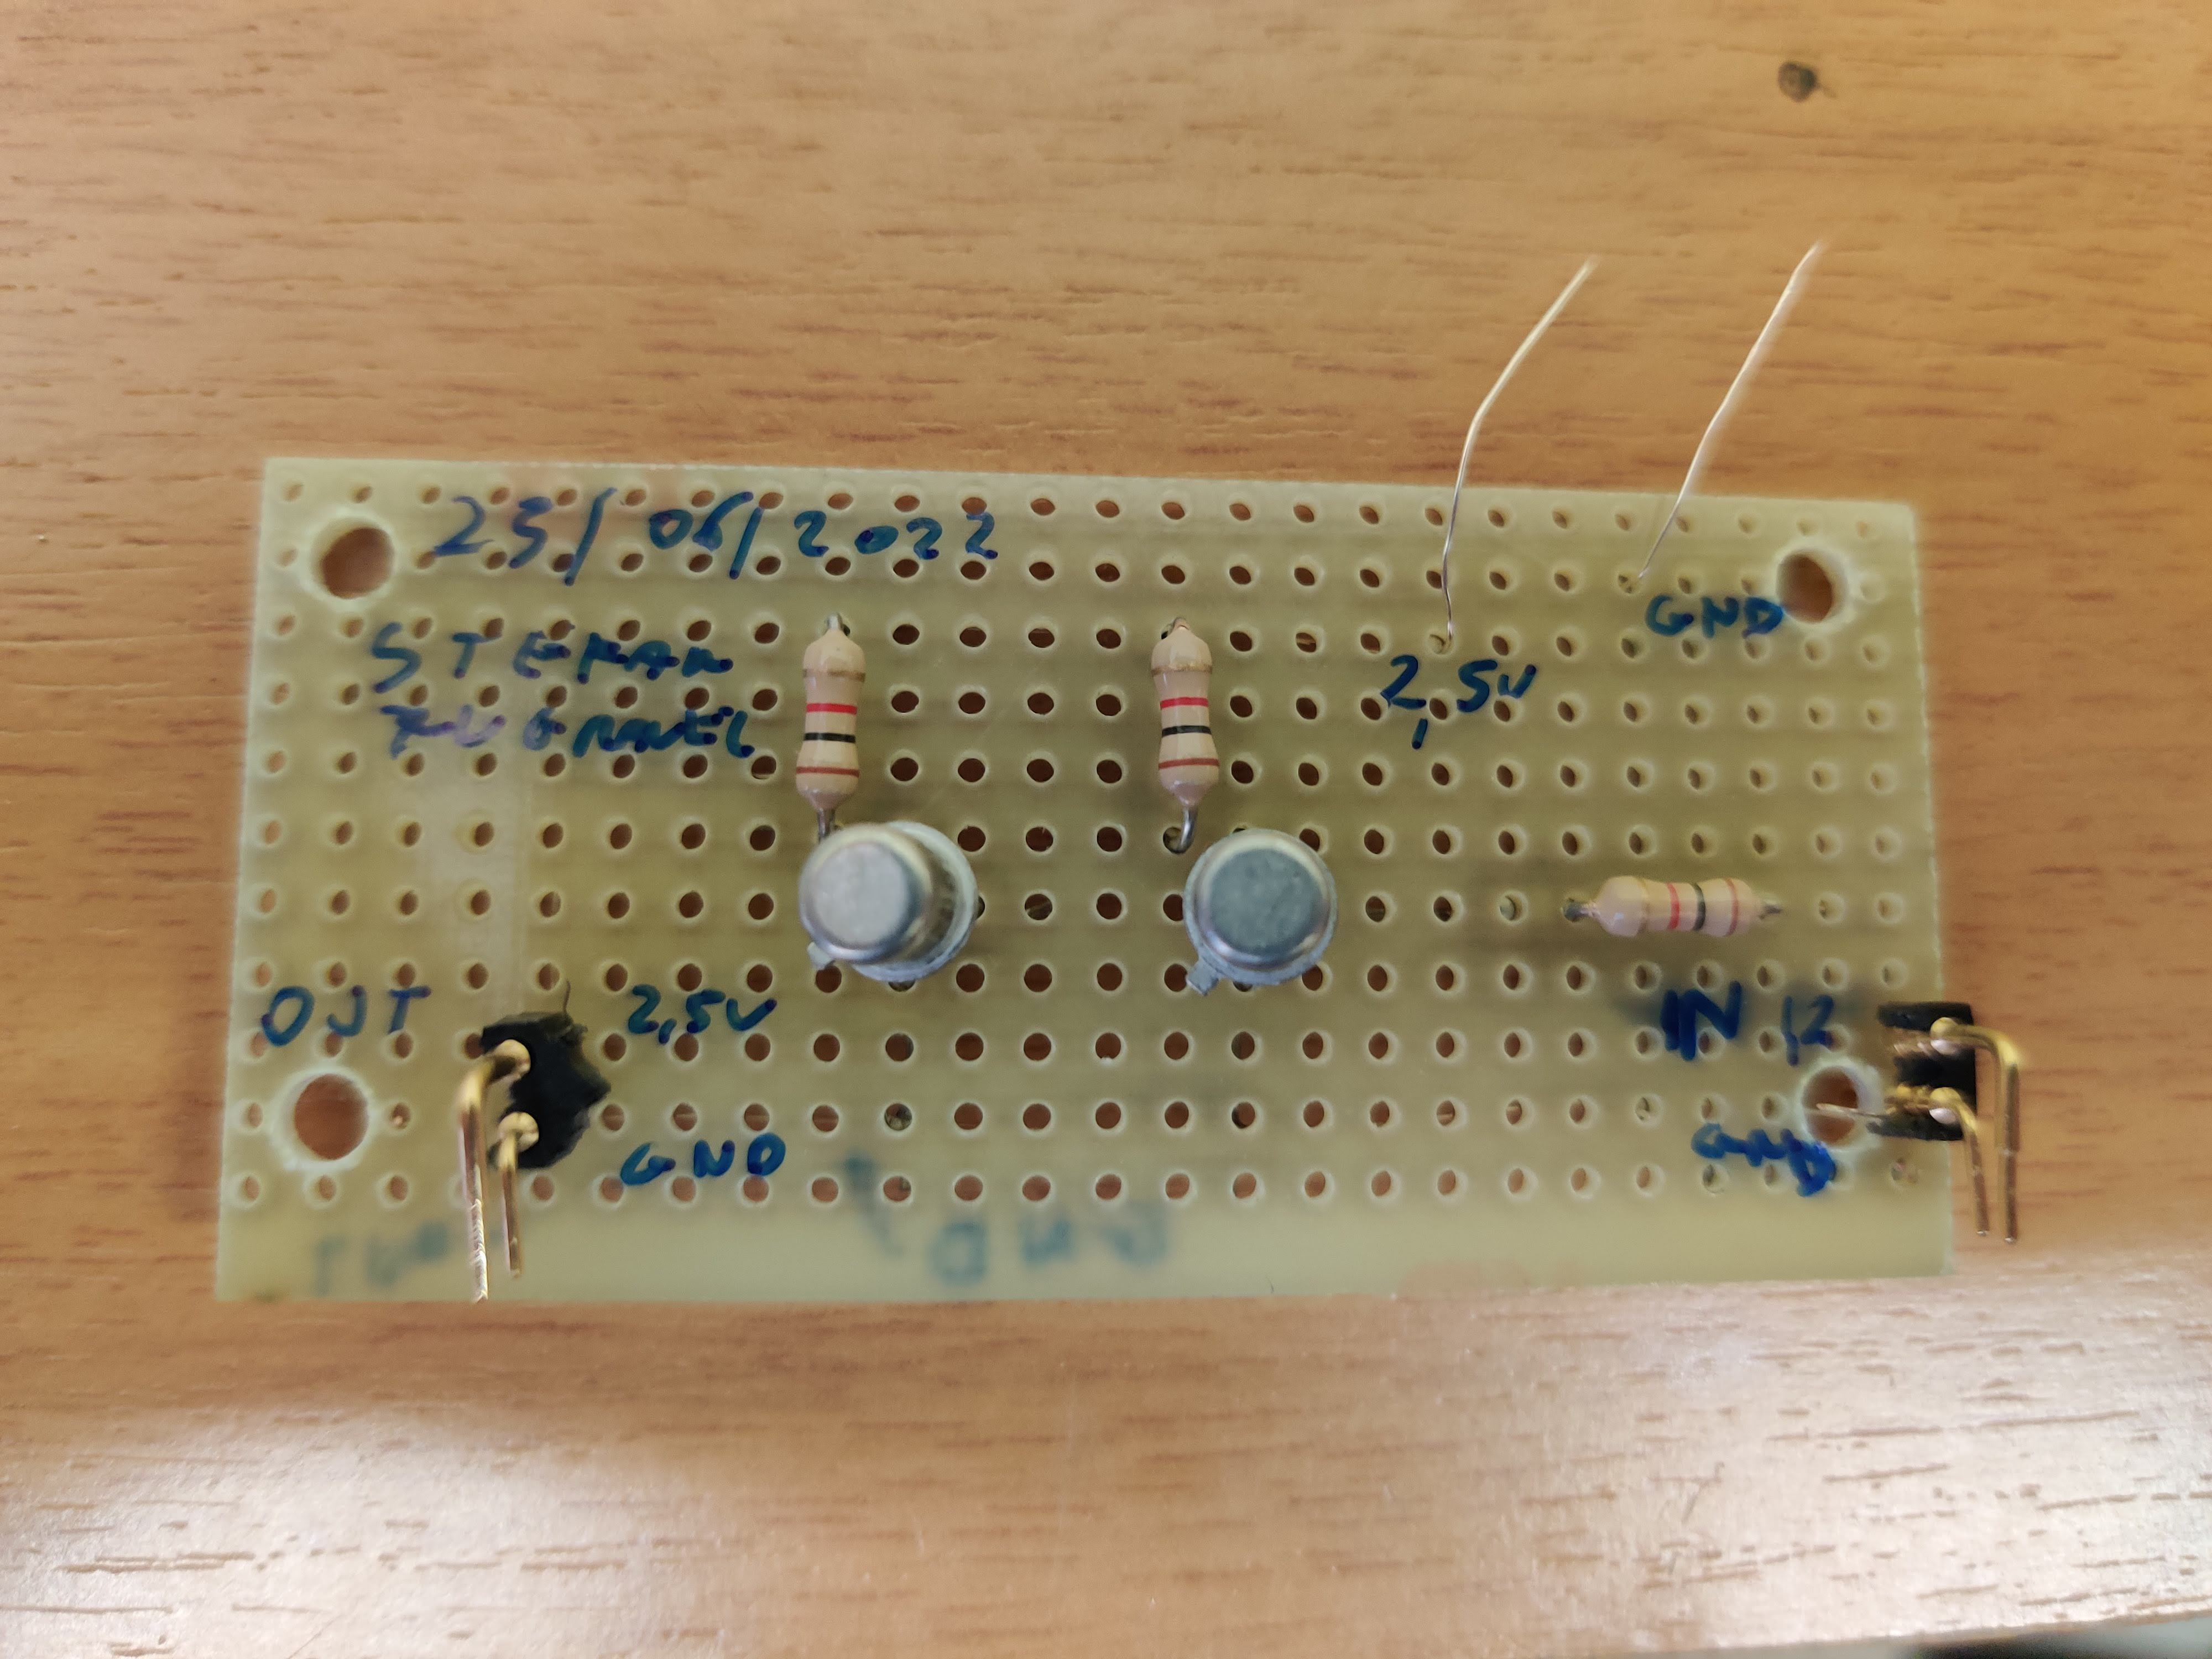
\includegraphics[width=0.8 \textwidth]{IMG/level_translator_front-min.jpg}
			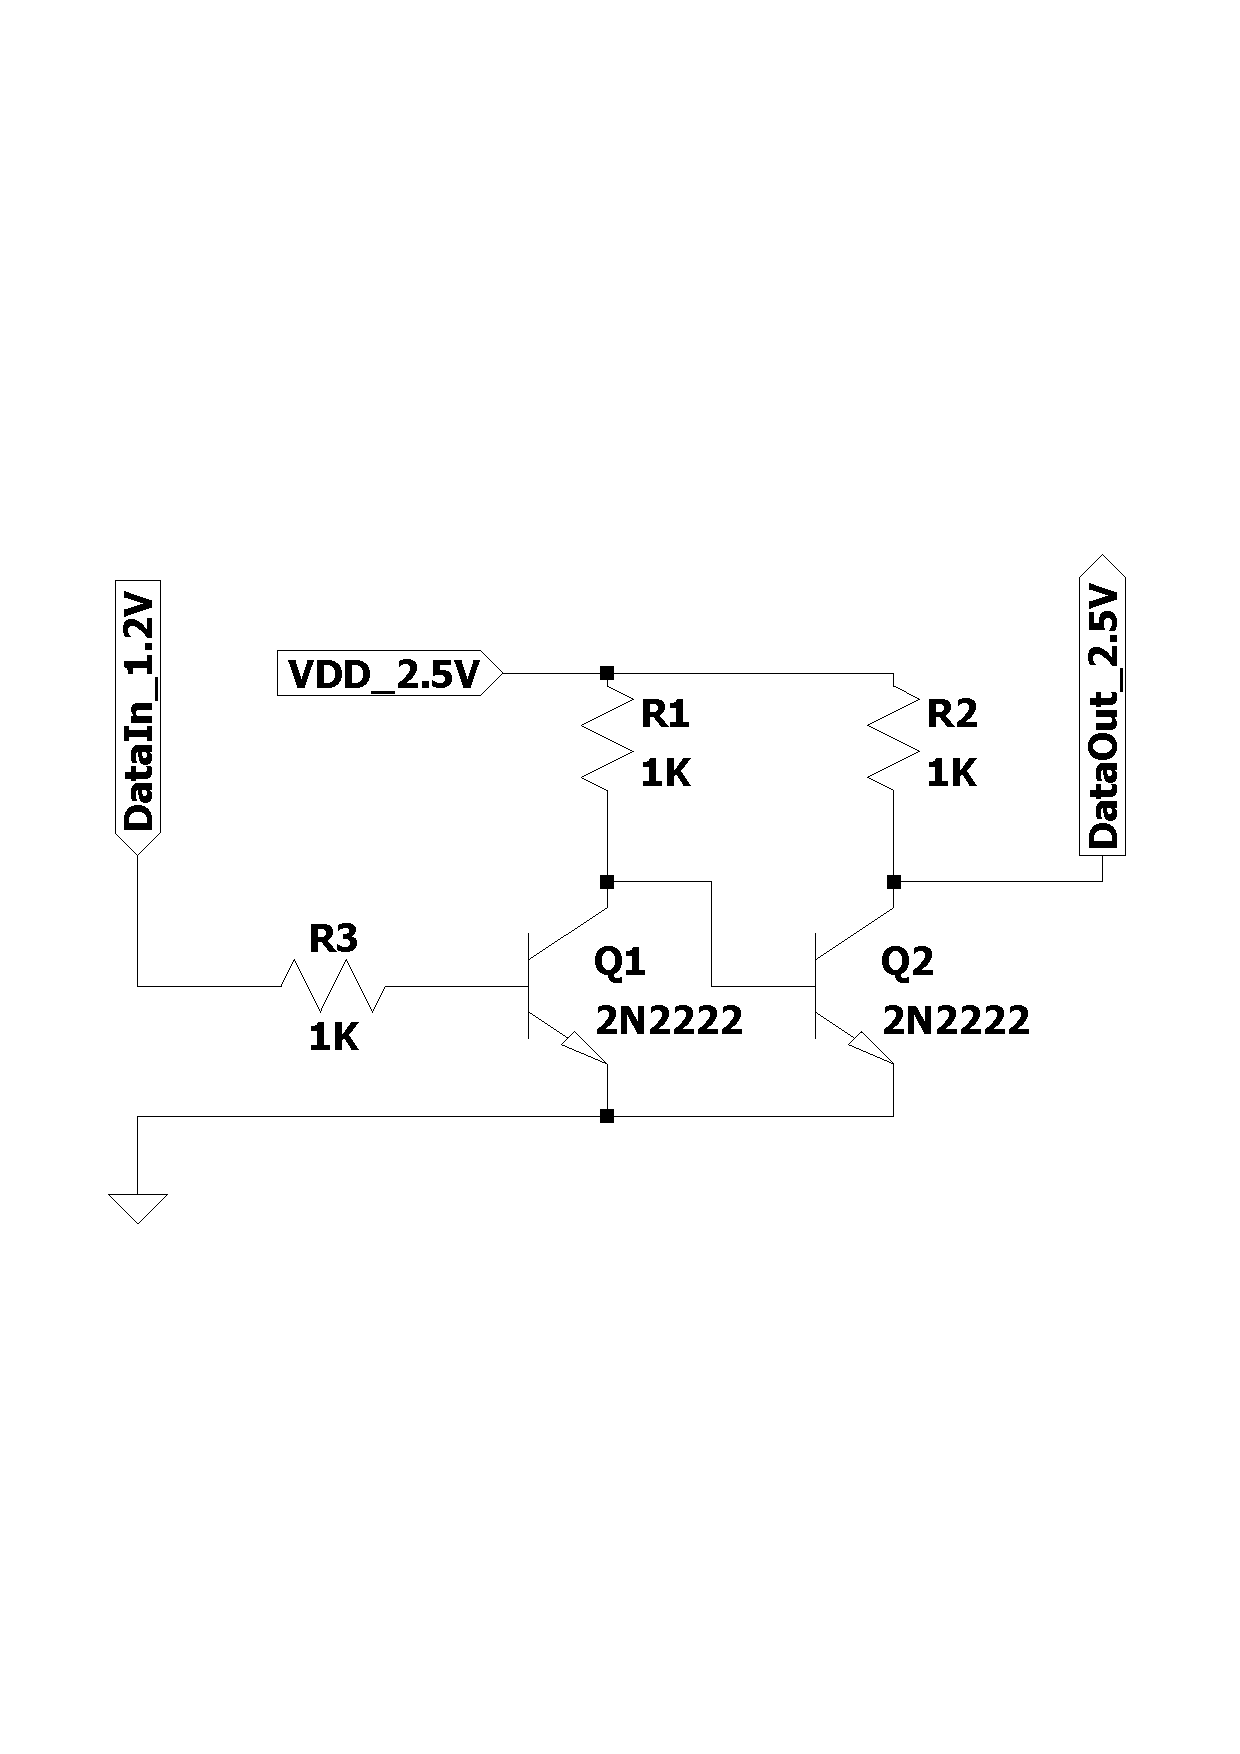
\includegraphics[width=0.8 \textwidth]{IMG/Diagram_cropped.pdf}
		\end{center}
		\column{0.65 \textwidth}
		\begin{center}
			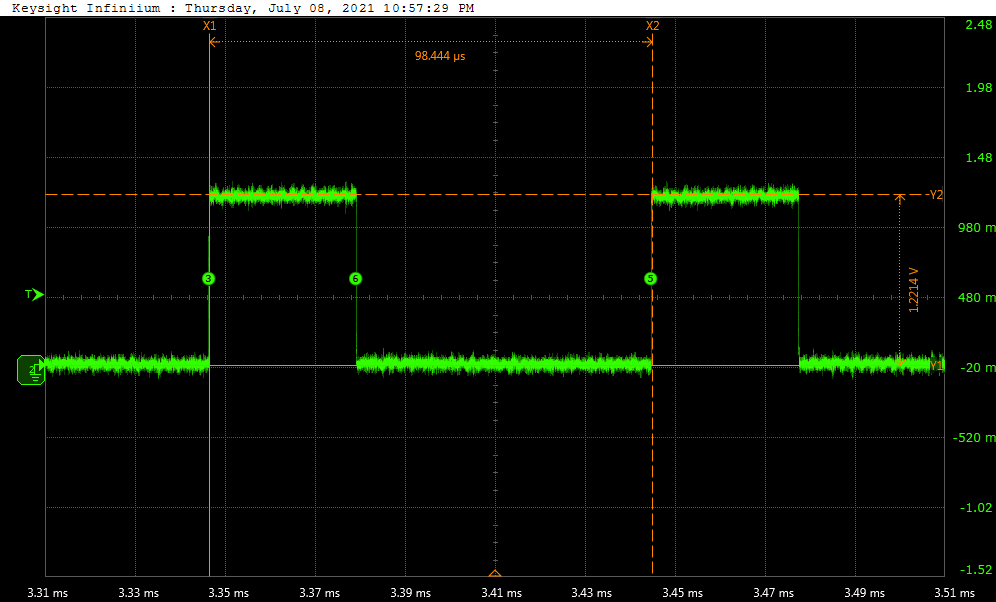
\includegraphics[width=0.5 \textwidth]{IMG/probe/09-08-2021_clock-specks.png}
		\end{center}
		\begin{itemize}
			\item ABACUS DACs I/O = CMOS \textbf{1.2}V single-ended
			\item FPGA I/O = CMOS \textbf{2.5}V single-ended
			\item Resistive \textbf{voltage divider}
			\item 2x \textbf{2N2222} NPN transistor in TO-18 package
			\item 3x \textbf{1}k$\Omega$ resistor 1/8W
		\end{itemize}
	\end{columns}
	\end{frame}

	\begin{frame}
		\frametitle{FPGA Firmware}
		\begin{columns}
			\column{0.5 \textwidth}
			\begin{center}
				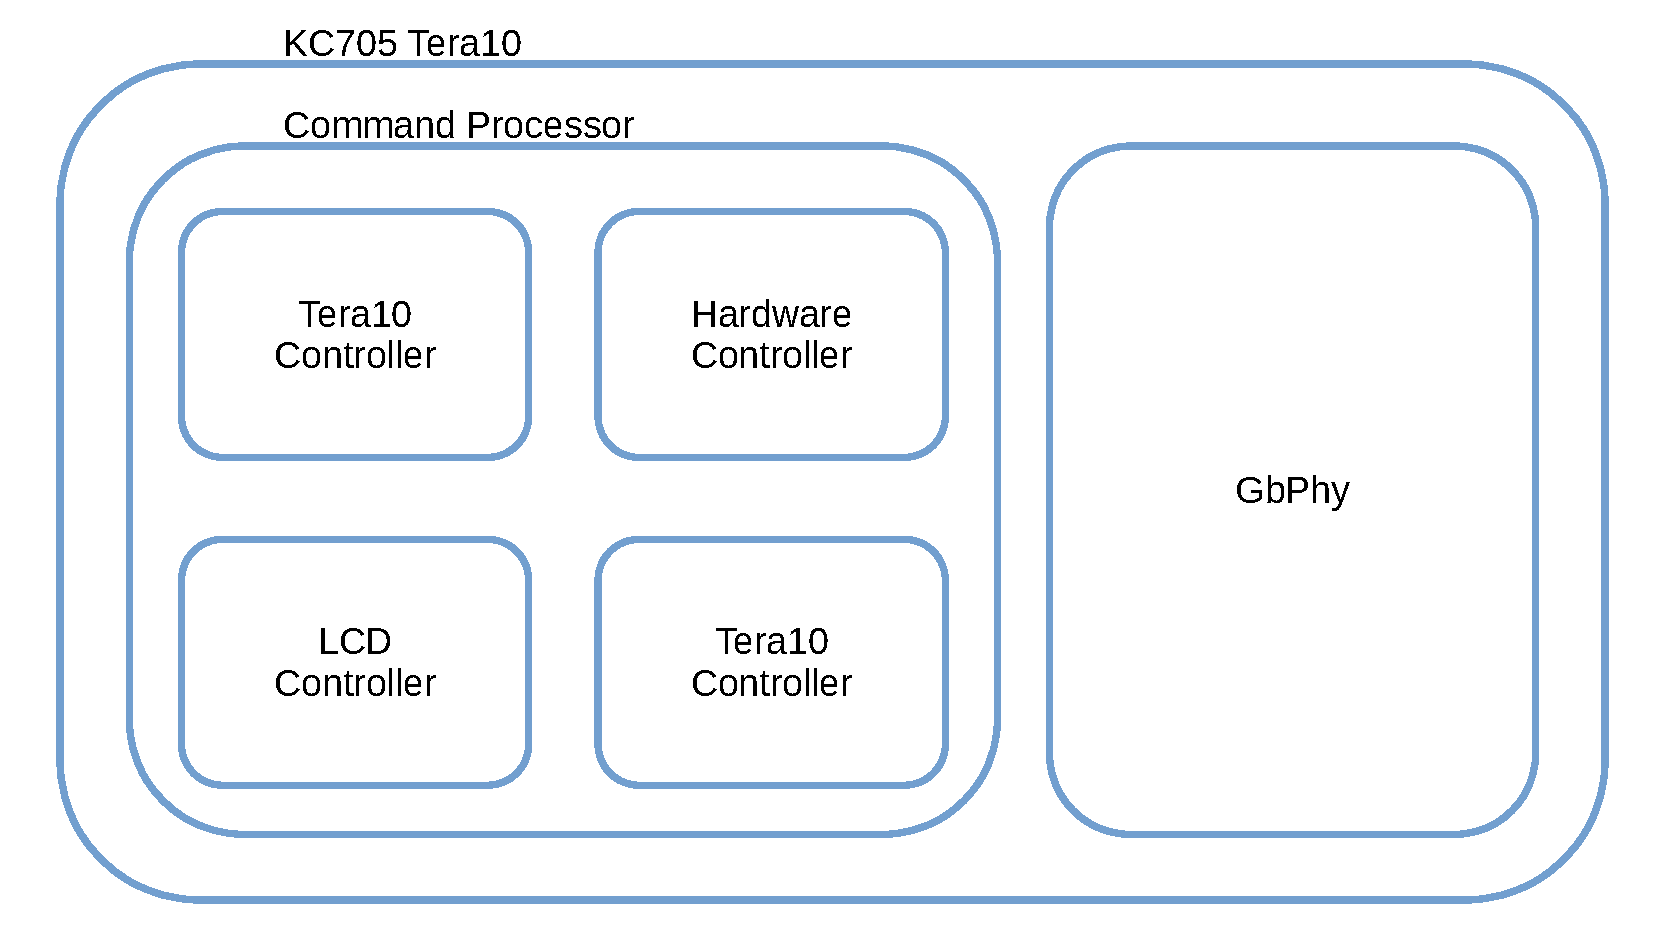
\includegraphics[width=1.0 \textwidth]{IMG/Tera10kc705.pdf}
			\end{center}
			\column{0.5 \textwidth}
			\begin{itemize}
				\item Original firmware written in \textbf{VHDL} by R.Wheadon (INFN-To) 
				\item GbPhy = Custom \textbf{UDP} Protocol
				\item LCD-Controller = display informations such~as:
					\begin{itemize}
						\item[$-$] Firmware version
						\item[$-$] Board number
						\item[$-$] Project name
					\end{itemize}
				\item Tera10-I/O = Input setup and counters
				\item Tera10-Controller = controls for reading and activate channels
				\item Hardware-Controller = setup internal and~external DACs
			\end{itemize}
		\end{columns}
	\end{frame}

	\begin{frame}
		\frametitle{ABACUS\_v2 internal DACs setup}	
		\begin{columns}
			\column{0.5 \textwidth}
			\begin{center}
				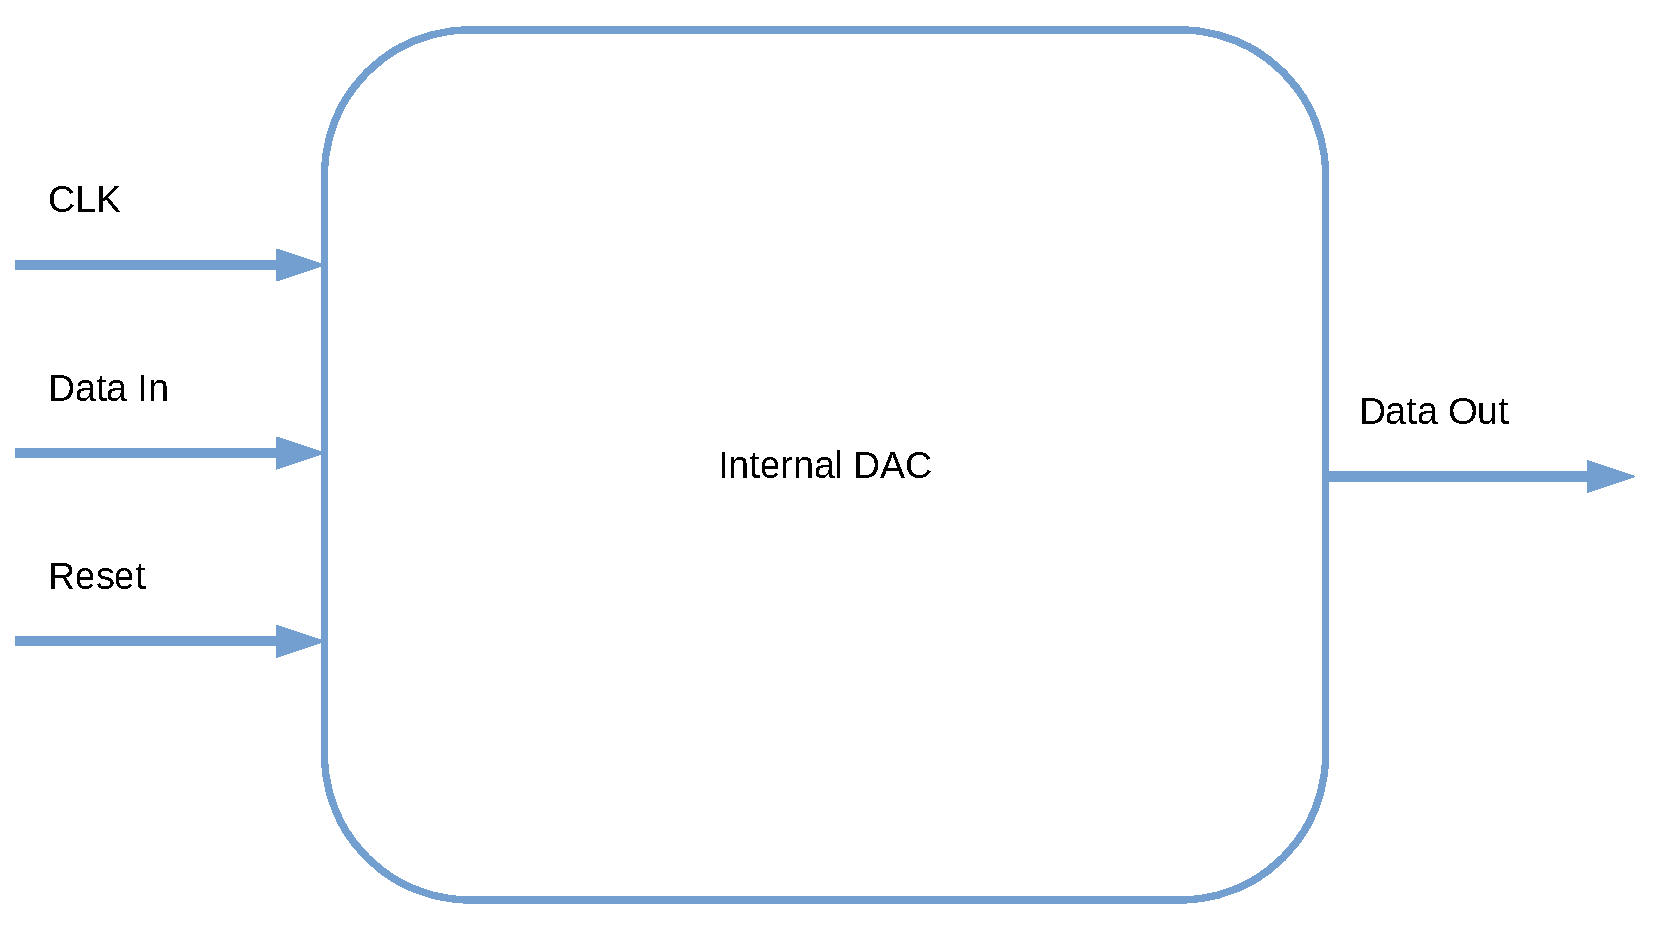
\includegraphics[width=0.7 \textwidth]{IMG/InternalDAC.pdf}
				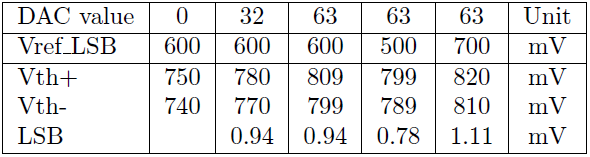
\includegraphics[width=0.7 \textwidth]{IMG/TableLSB.PNG}
			\end{center}
			\textbf{LSB} value $\approx$ 0.94 mV for \textbf{Vref\_LSB} = 600~mV
			\column{0.5 \textwidth}
			{\color{blue} Internal DAC setup}
			\begin{itemize}
				\item Initialization sequence \textbf{0xA5A5}= 
				\newline
				1010-0101-1010-0101
				\item \textbf{16bit words}= \newline 2bit command + 6bit address + 8bit data
				\begin{itemize}
					\item \textbf{command}
					\begin{itemize}
						\item \textbf{11} = write
						\item \textbf{10} = read
					\end{itemize}
					\item \textbf{address}
					\begin{itemize}
						\item \textbf{5bit} address from \textbf{0} to \textbf{23}
						\item \textbf{LSB} is Vth$\pm$ (not used for now)
					\end{itemize}
					\item \textbf{data}
					\begin{itemize}
						\item \textbf{2MSB} not used
						\item \textbf{6LSB} data for the internal DAC \newline from \textbf{0} to \textbf{63}
					\end{itemize}
				\end{itemize} 
			\end{itemize}
		\end{columns}
	\end{frame}

	\begin{frame}
	\frametitle{Firmware - DATA}
	\begin{itemize}
		\item The \textbf{FPGA} communicates with the PC using Ethernet/UDP (\textbf{U}ser \textbf{D}atagram \textbf{P}rotocol) implemented in the \textbf{GbPhy} project
		\item Each UDP packet is \textbf{64} bit long $\rightarrow$ \textbf{32} bit used by GbPhy and \textbf{32} bit of user data
		\item \textbf{32} bit data =
		\begin{itemize}
			\item \textbf{4} bit $\rightarrow$ firmware target (0x4 for HW command)
			\item \textbf{8} bit $\rightarrow$ firmware command (0x11 for DAC config)
			\item \textbf{20} bit $\rightarrow$ firmware data
		\end{itemize}
		\item \textbf{20} bit firmware data =
		\begin{itemize}
			\item \textbf{3} bit not used
			\item \textbf{2} bit baseline DAC command
			\item \textbf{6} bit baseline DAC address
			\item \textbf{8} bit baseline DAC data
			\item \textbf{1} bit baseline DAC selecet (each FPGA can control 2 chips)
		\end{itemize}
		\item To perform a Read/write operation the initialization sequence must be sent first\newline every time
	\end{itemize}
	\end{frame}

	\begin{frame}[fragile]
		\frametitle{Firmware - FSM for internal DAC configuration}
		\begin{columns}
			\column{0.5 \textwidth}
			\begin{center}
				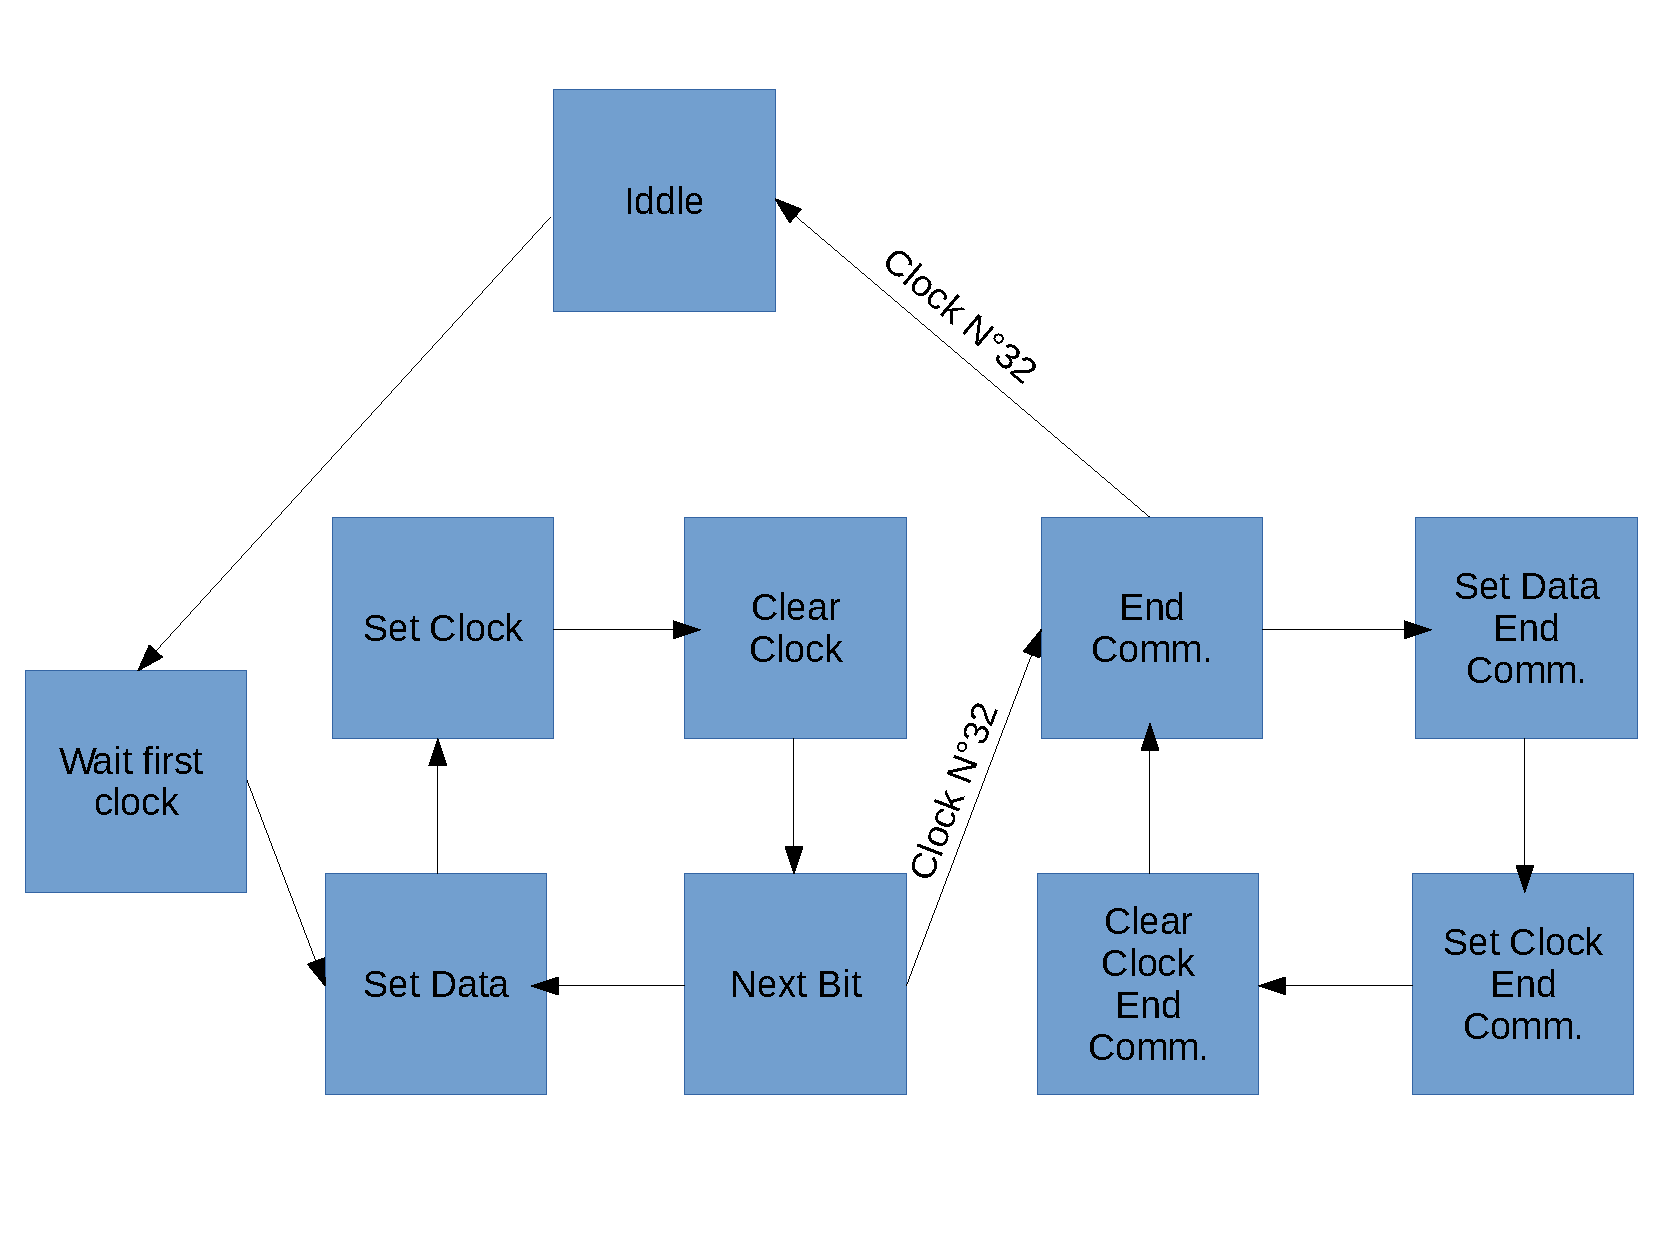
\includegraphics[width=0.95 \textwidth]{IMG/FSM.pdf}
			\end{center}
			\column{0.5 \textwidth}
			\begin{itemize}
				\item FSM (\textbf{F}inite \textbf{S}tate \textbf{M}achine): states for the~serial data communication
				\item \textbf{32} clock pulses sending data=
				\begin{itemize}
					\item \textbf{16} bit = initialization sequence
					\item \textbf{16} bit = data
				\end{itemize}
				\item \textbf{32} bit waiting the response
				\item Set Data End Communication is always zero
			\end{itemize}
		\end{columns}
	\end{frame}


	\begin{frame}
	\frametitle{Example Xilinx Vivado simulation}
		\begin{center}
			Finite State Machine \\
			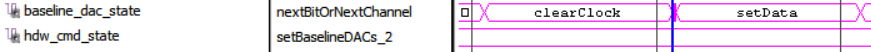
\includegraphics[width=0.9 \textwidth]{IMG/Simulation1.png}
			\newline
			write internal DAC channel 4 \\
			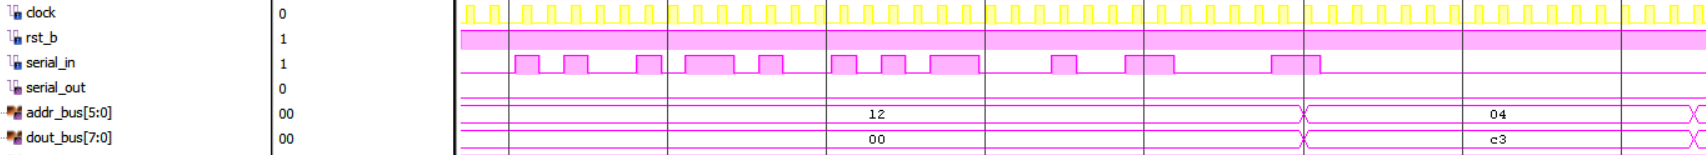
\includegraphics[width=0.9 \textwidth]{IMG/Simulation3.png}
			\newline
			read internal DAC channel 4 \\
			{\hspace*{-5mm}
			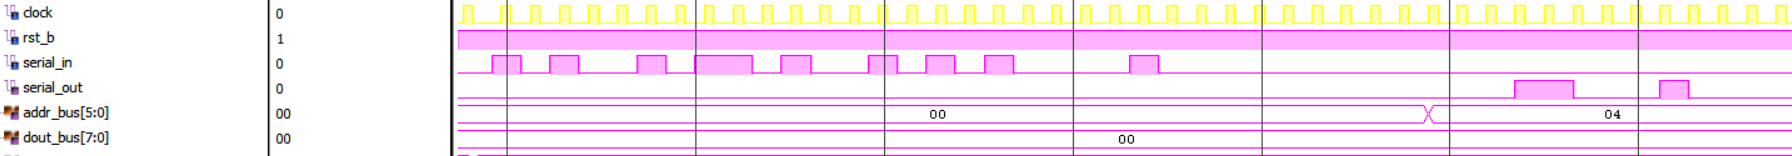
\includegraphics[width=0.9 \textwidth]{IMG/Simulation4.png}}
		\end{center}
	\begin{itemize}
		\item The DAC behaviour is \textbf{simulated} by a \textbf{Verilog} module
	\end{itemize}
	\end{frame}

	
	\begin{frame}
	\frametitle{Writing Internal DACs for threshold-tuning}
	\begin{columns}
		\column{0.5 \textwidth}
	{\color{blue} Input}
	\begin{itemize}
		\item Initialization sequence = 0xA5A5
		\item Write command = 11 
		\item Address = 100010 = 10001-0 = channel 17
		\item Data    = 00111111 = 63
	\end{itemize}
	\column{0.5 \textwidth}
	{\color{blue} Clock Specs}
	\begin{itemize}
		\item Period = \textbf{98.44} $\mu$s
		\item Duty cycle \textbf{33}\%
		\item Packet duration $\approx$ \textbf{6.4} ms
	\end{itemize}
	\end{columns}
	\begin{columns}
		\column{0.75 \textwidth}
		\begin{center}
			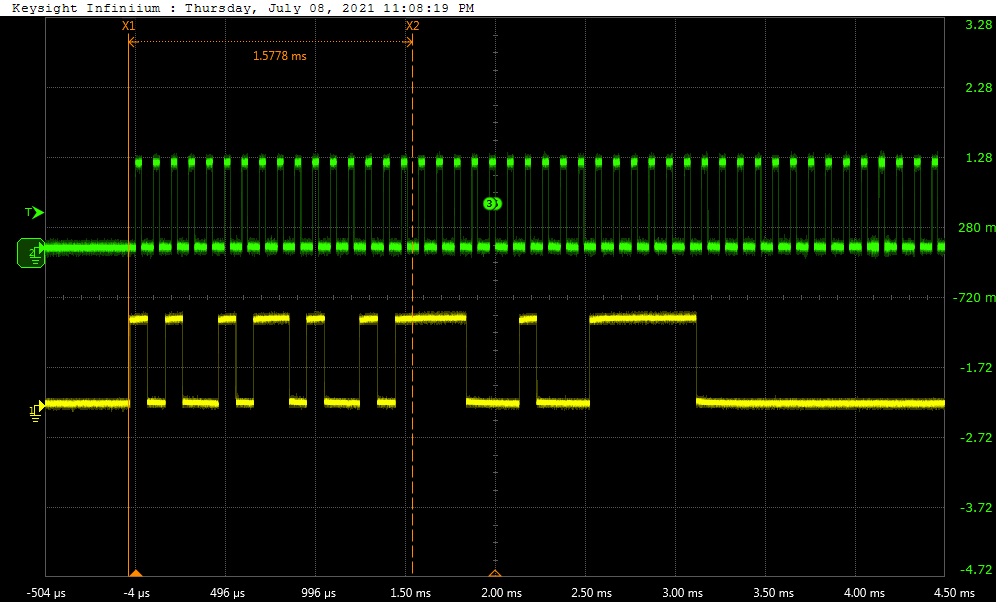
\includegraphics[width=0.667 \textwidth]{IMG/probe/09-08-2021_ch17-write63-baselinedac1.png}
		\end{center}
		\column{0.2 \textwidth}
		\hspace{-20mm} \vspace{8mm}
		{\color{green} clock signal}\\
		\hspace{-20mm} \vspace{-4mm}
		{\color{yellow} input data}
		\column{0.05 \textwidth}
	\end{columns}
	\end{frame}

	
	\begin{frame}
	\frametitle{Reading Internal DACs for threshold-tuning}
	\begin{columns}
		\column{0.5 \textwidth}
		{\color{blue} Input}
		\begin{itemize}
			\item Initialization sequence = 0xA5A5
			\item Read command = 10 
			\item Address = 001010 = 00101-0 = channel 05
			\item Data    = 00000000
		\end{itemize}
		\column{0.5 \textwidth}
		{\color{blue} Output}
		\begin{itemize}
			\item 11 = read
			\item 001010 = 00101-0 = channel 05
			\item 00110101 = 53
		\end{itemize}
	\end{columns}
	\begin{columns}
		\column{0.75 \textwidth}
		\begin{center}
			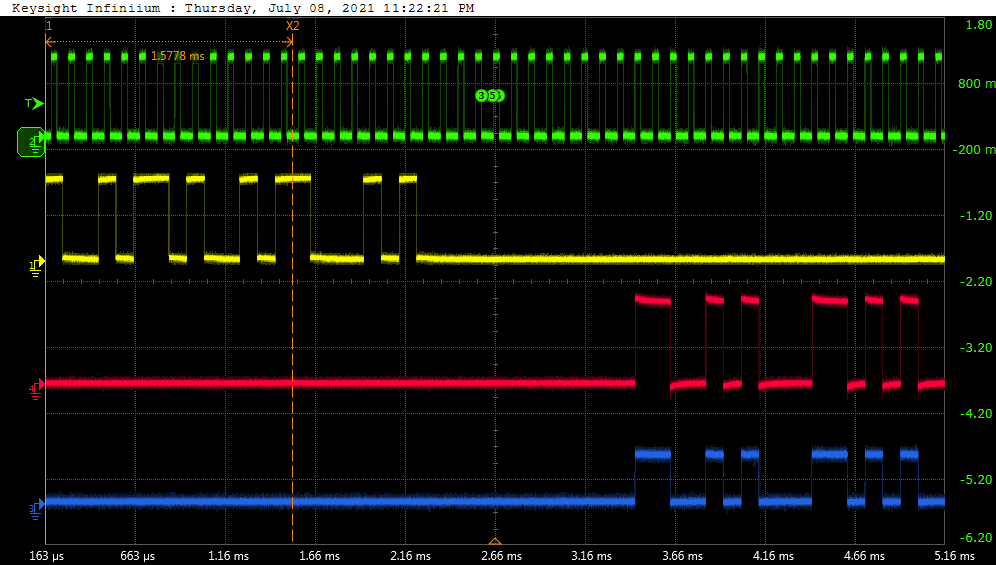
\includegraphics[width=0.667 \textwidth]{IMG/probe/09-08-2021_ch05-read53-baselinedac1.png}
		\end{center}
		\column{0.2 \textwidth}
			\hspace{-20mm} \vspace{5mm}
			{\color{green} clock signal} \\
			\hspace{-20mm} \vspace{5mm}
			{\color{yellow} input data} \\
			\hspace{-20mm} \vspace{5mm}
			{\color{red} output data 2.5V} \\
			\hspace{-20mm} \vspace{-7mm}
			{\color{blue} output data 1.2V}
		
		\column{0.05 \textwidth} 
	\end{columns}
		
	\end{frame}

%%%%%%%%%%%%%%%%%%%%%%%%%%%%%%%%%%%%%%%%%%%%%%%%%%%%%%%%%%%%%%%%%%%%%%%%%%%%%%%%%%%%%%%%



	\section{Results}
	
	\begin{frame}[plain, noframenumbering]
	%\frametitle{results}
	\begin{center}
		{\Huge \fontfamily{qtm}\selectfont \color{blue} \textbf{Preliminary results}}
	\end{center}
	\end{frame}
	
	\begin{frame}
	\frametitle{Threshold scan}
		\begin{itemize}
			\item Internal DACs configuration allows to adjust the threshold for each channel
			\item Example: ch \textbf{1}, global threshold scan with fixed injected charge and \textbf{10} kHz test pulse rate
			\item {\color{blue}Blue} curve: trimming DAC code= \textbf{0} = \textbf{0x00}
			\item {\color{green}Green} curve: trimming DAC code= \textbf{63} = \textbf{0x3F}
			\item S-curves shifted as expected  
		\end{itemize}	
		\begin{center}
			\vspace*{-5mm} 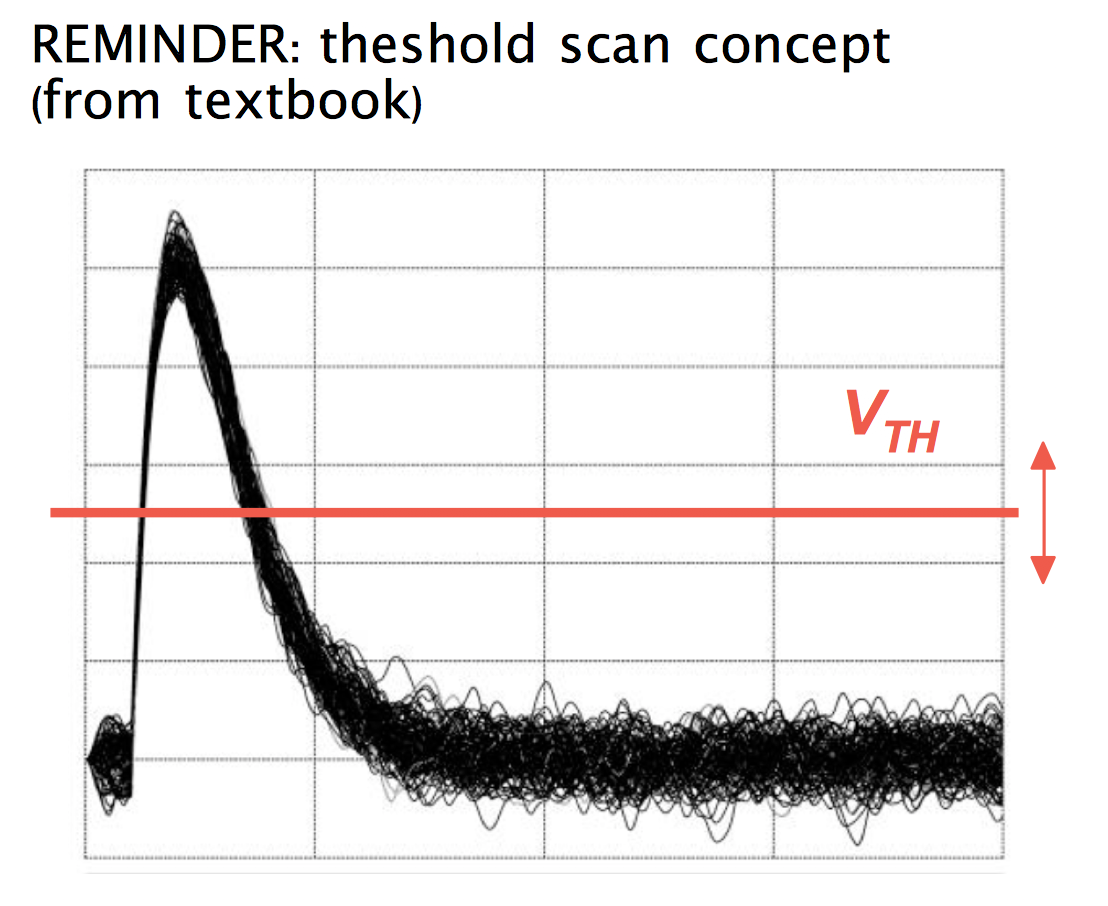
\includegraphics[width=0.35 \textwidth]{IMG/tscan_sketch.png}
			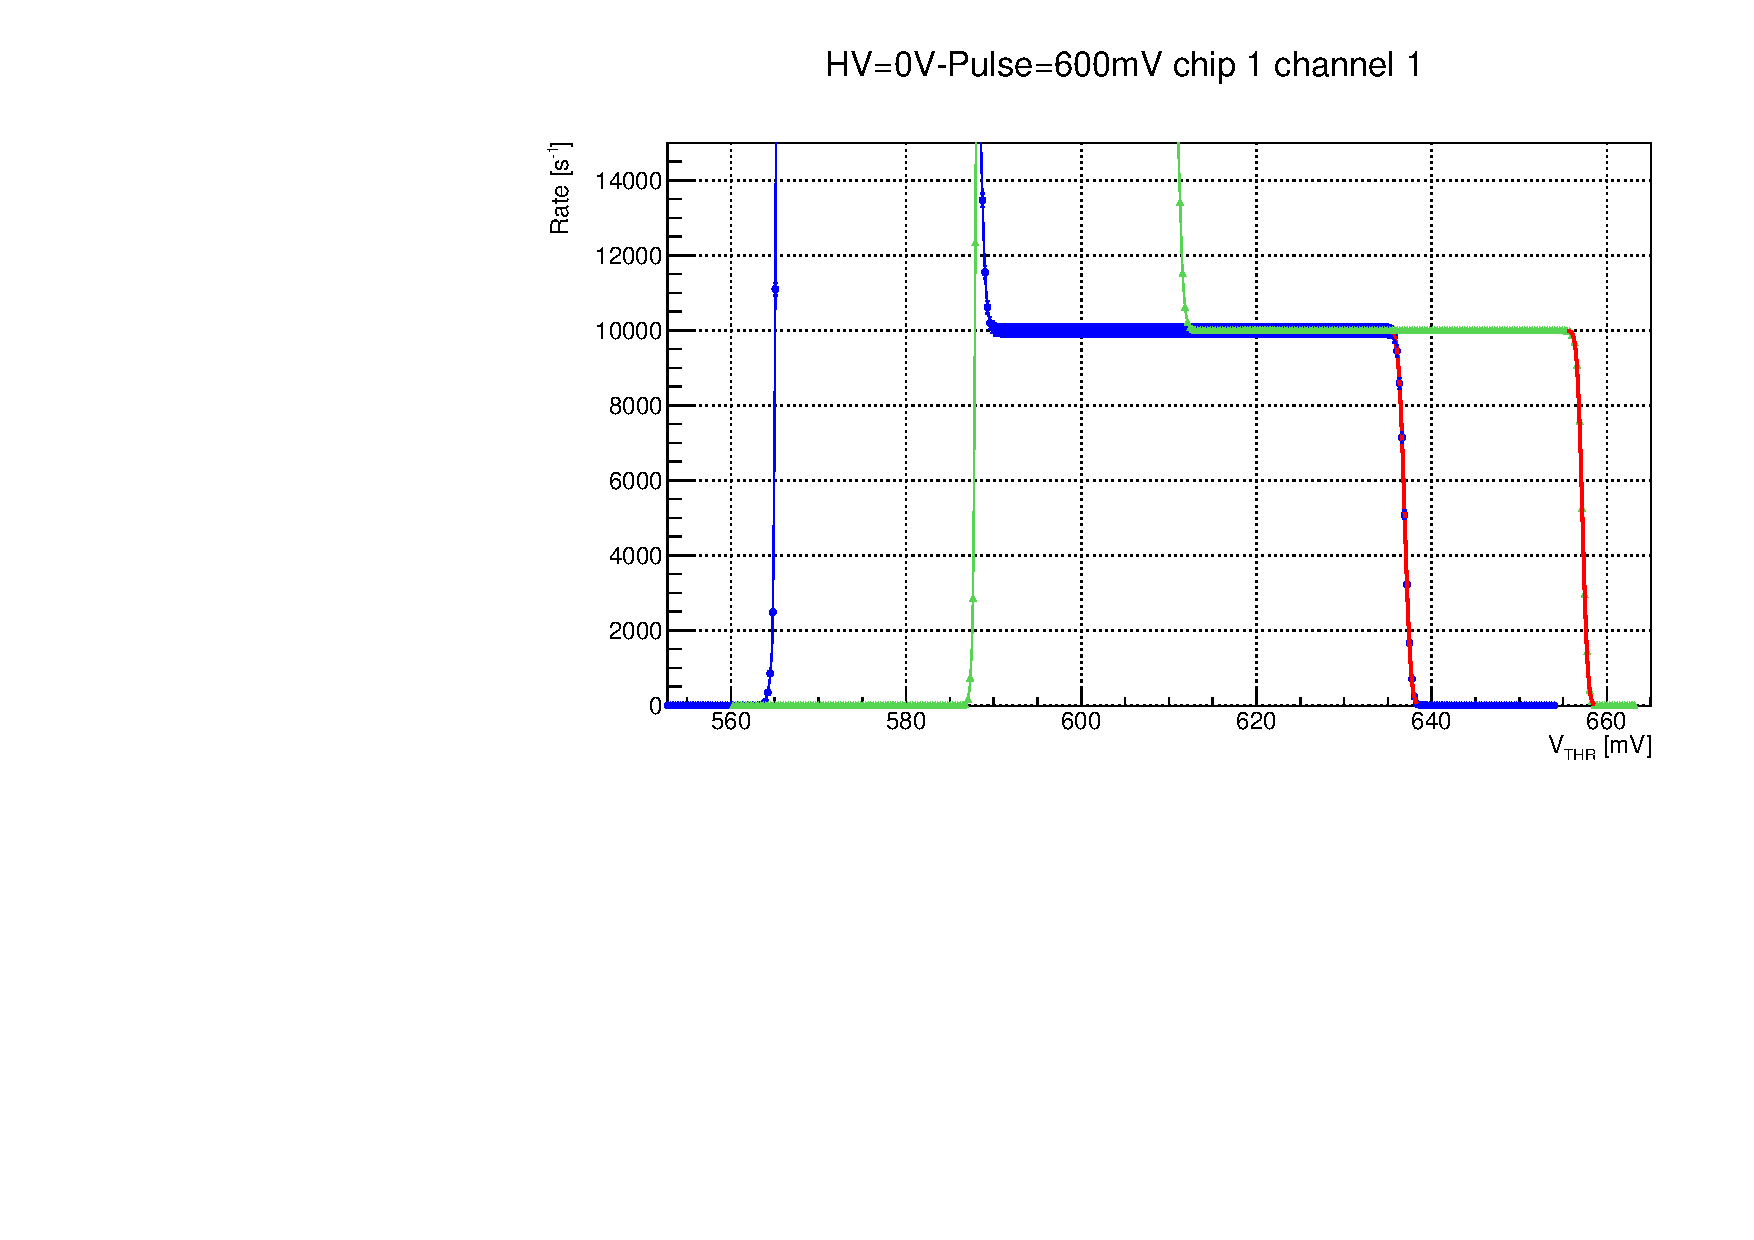
\includegraphics[width=0.55 \textwidth]{IMG/ThScan_ch0.pdf}
		\end{center}
		
	\end{frame}

	%\begin{frame}
	%\frametitle{Pedestal distribution-1}
	%\begin{itemize}
	%	\item Pedestal voltage value for odd channels
	%	\item {\color{blue}Blue} dots with baseline dac=\textbf{63}
	%	\item {\color{red}Red} dots with baseline dac=\textbf{0}
	%\end{itemize}
	%\begin{center}
	%	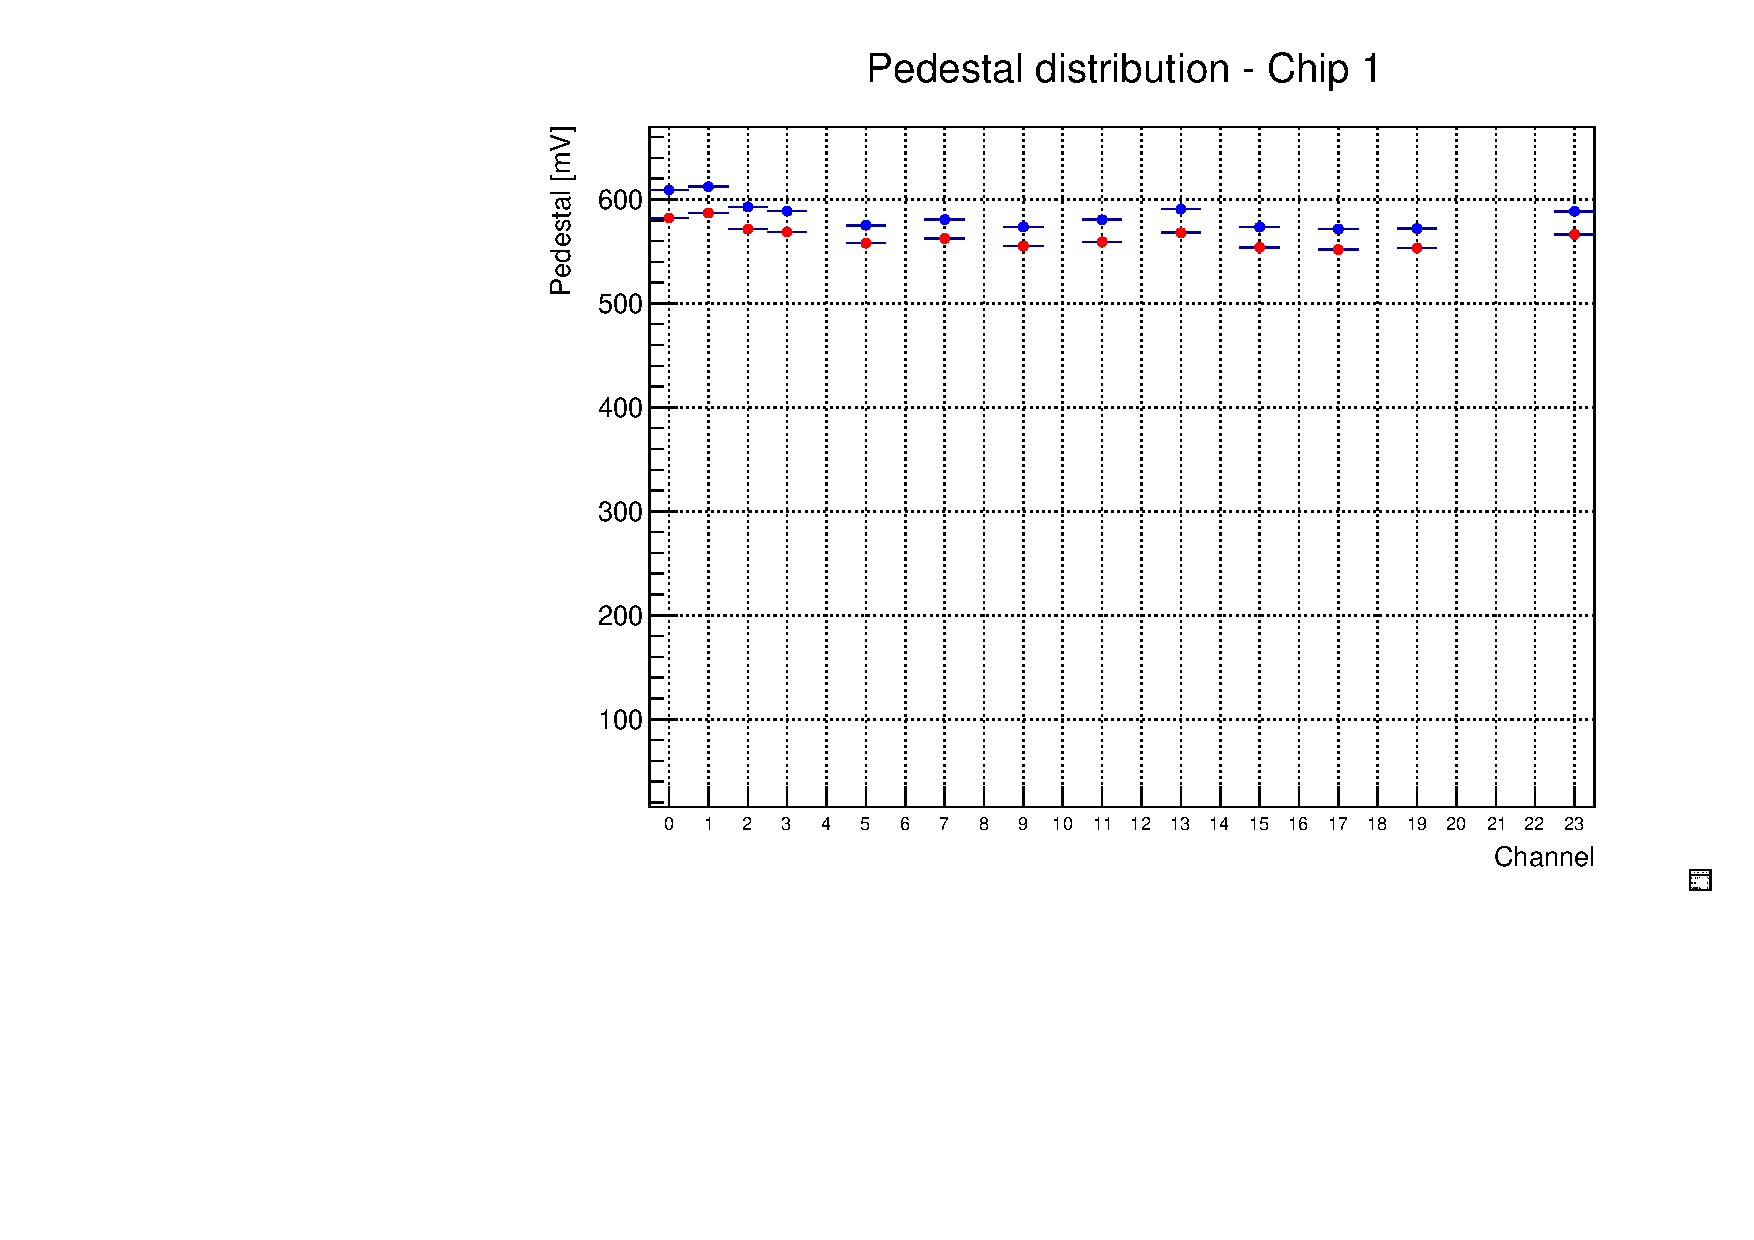
\includegraphics[width=0.59 \textwidth]{data/DAC_V_REF_600mV.pdf}
	%\end{center}
	%
	%\end{frame}

	\begin{frame}
	\frametitle{Pedestal distribution}
	\begin{itemize}
		\item Extrapolated DC \textbf{CSA} output voltage values for selected channels
		\item {\color{blue}Blue} dots: trimming DAC code= \textbf{0} = \textbf{0x00}
		\item {\color{green}Green} dots: trimming DAC code= \textbf{63} = \textbf{0x3F}
		\item Average $\Delta V\approx$ 22 mV
	\end{itemize}
	\begin{center}
		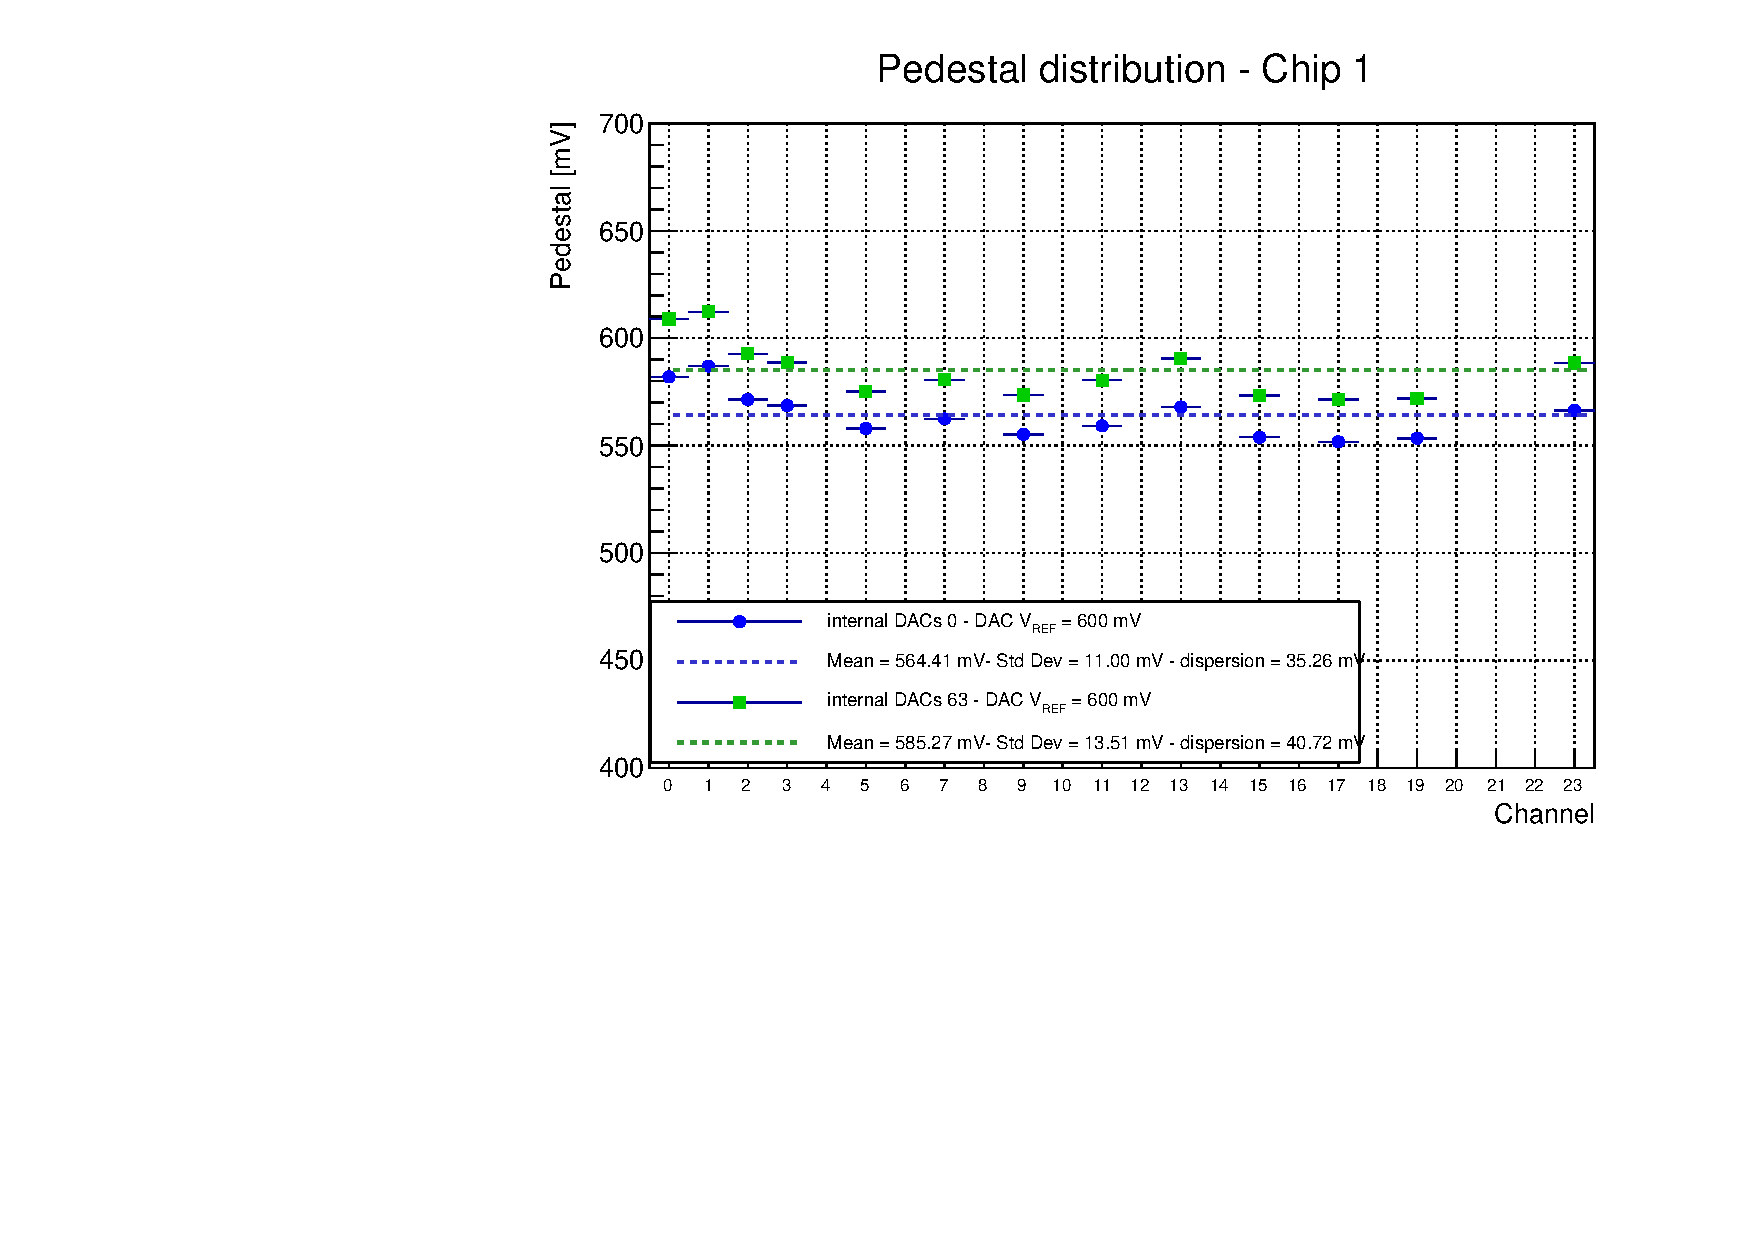
\includegraphics[width=0.55 \textwidth]{data/DAC_V_REF_600mV-Copia.pdf}
	\end{center}
	
\end{frame}

%%%%%%%%%%%%%%%%%%%%%%%%%%%%%%%%%%%%%%%%%%%%%%%%%%%%%%%%%%%%%%%%%%%%%%%%%%%%%%%%%%%%%%%%
	\section{Conclusions}
	
	\begin{frame}
	\frametitle{Conclusions and To Do List}
	\begin{center}
		{\color{blue}\textbf{Conclusions}}
	\end{center}
		\begin{itemize}
			\item New \textbf{FPGA} firmware extensions added for the configuration and readout of the ABACUS\_v2 chip
			\item \textbf{Successfully} tested with simulations and in laboratory
		\end{itemize}
	
	\begin{center}
		{\color{blue}\textbf{Future work and additions to the FPGA firmware}}
	\end{center}
		\begin{itemize}
			\item Internal DACs \textbf{characterization} and verification of their \textbf{linearity}
			\item Addition of a \textbf{latch} in order to save into a \textbf{register} the current state of every counter 
			\item Addition of a \textbf{timestamp} in order to obtain a more accurate rate calculation 
			%\item Addition of a configurable \textbf{mask} to calculate via firmware the \textbf{sum} of only certain selected channels 		
		\end{itemize}
			\vspace{1 cm}
		\begin{center}
			\textbf{Thanks for the attention!!}
		\end{center}	
	\end{frame}

	\begin{frame}[noframenumbering]
	\frametitle{References}
	{\scriptsize 
	\begin{thebibliography}{00}
		\bibitem{1}www.researchgate.net/figure/Dose-depth-curve-for-monoenergetic-photons-protons-and-carbon-ions-courtesy-of-GSI\textunderscore fig1\textunderscore283521369
		\newline
		\bibitem{2}www.intechopen.com/books/novel-prospects-in-oxidative-and-nitrosative-stress/oxidative-stress-in-hadrontherapy
		\newline
		\bibitem{3}www.semanticscholar.org/paper/A-Millimeter-Scale-Single-Charged-Particle-for-Lee-Scholey/ae955a07a42e9c124a8473357cd485b0b9928090
		\newline
		\bibitem{4}www.semanticscholar.org/paper/Low-Gain-Avalanche-Detectors-(LGAD)-for-particle-Moffat-Bates/0477d7bc2c9a3b26ad776874598f56d7d5b54c45
		\newline
		\bibitem{5}MoveIt v2 design document, Giovanni Mazza, January 15, 2021
	\end{thebibliography} }
	\end{frame}

%%%%%%%%%%%%%%%%%%%%%%%%%%%%%%%%%%%%%%%%%%%%%%%%%%%%%%%%%%%%%%%%%%%%%%%%%%%%%%%%%%%%%%%%
	\section{Backup}
	
	\begin{frame}[plain, noframenumbering]
	\begin{center}
		{\Huge \fontfamily{qtm}\selectfont \color{blue} \textbf{Backup}}
	\end{center}
	\end{frame}
	
	\begin{frame}[noframenumbering]
	\frametitle{Additional Graphs}
	\begin{columns}
		\column{0.3 \textwidth}
		\begin{center}
			\begin{figure}
				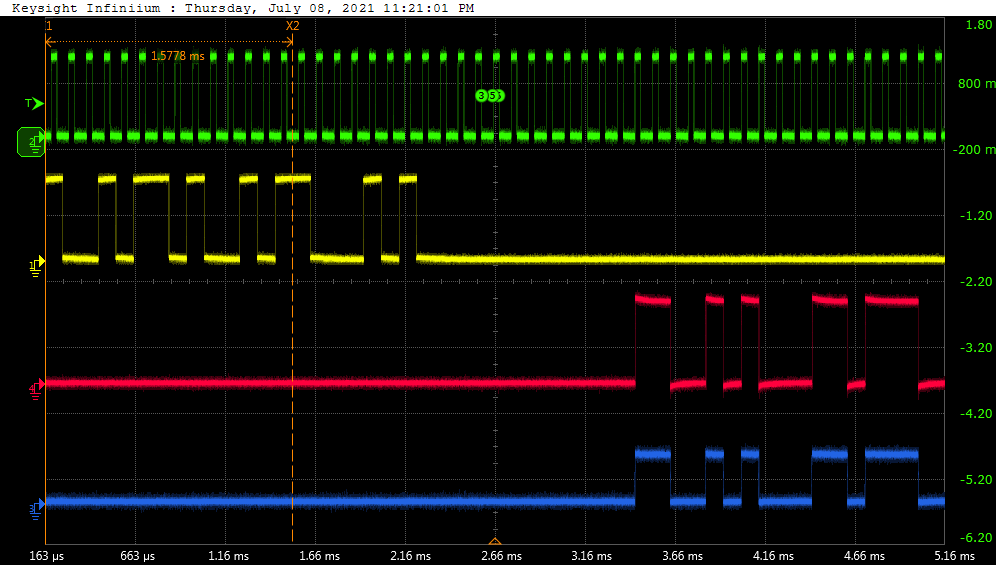
\includegraphics[width=0.95 \textwidth]{IMG/probe/09-08-2021_ch05-read55-baselinedac1.png}
				\caption{\centering{\tiny ch05-read55}}
			\end{figure}
			\begin{figure}
				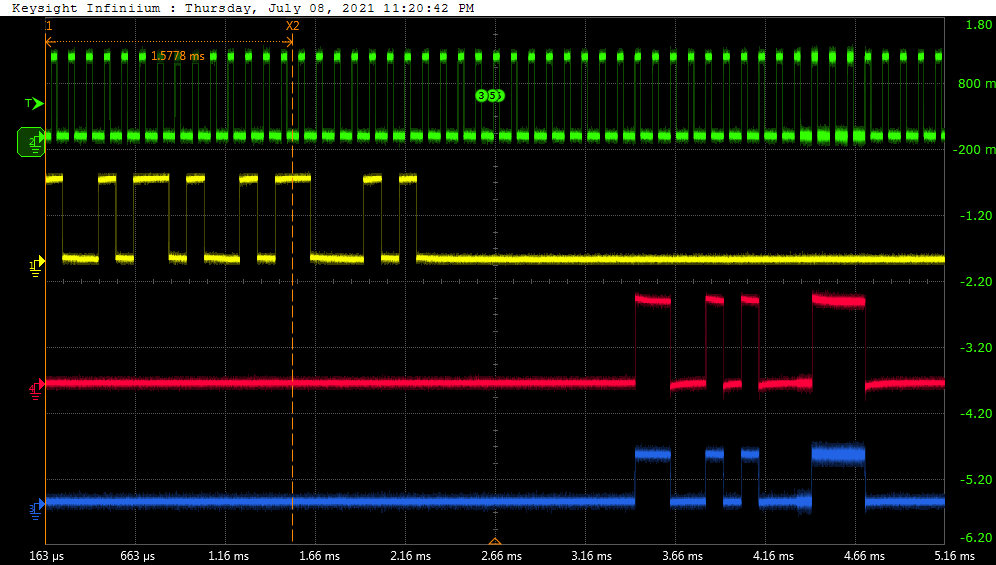
\includegraphics[width=0.95 \textwidth]{IMG/probe/09-08-2021_ch05-read56-baselinedac1.png}
				\caption{\centering{\tiny ch05-read56}}
			\end{figure}		
		\end{center}
		\column{0.3 \textwidth}
		\begin{center}
			\begin{figure}
				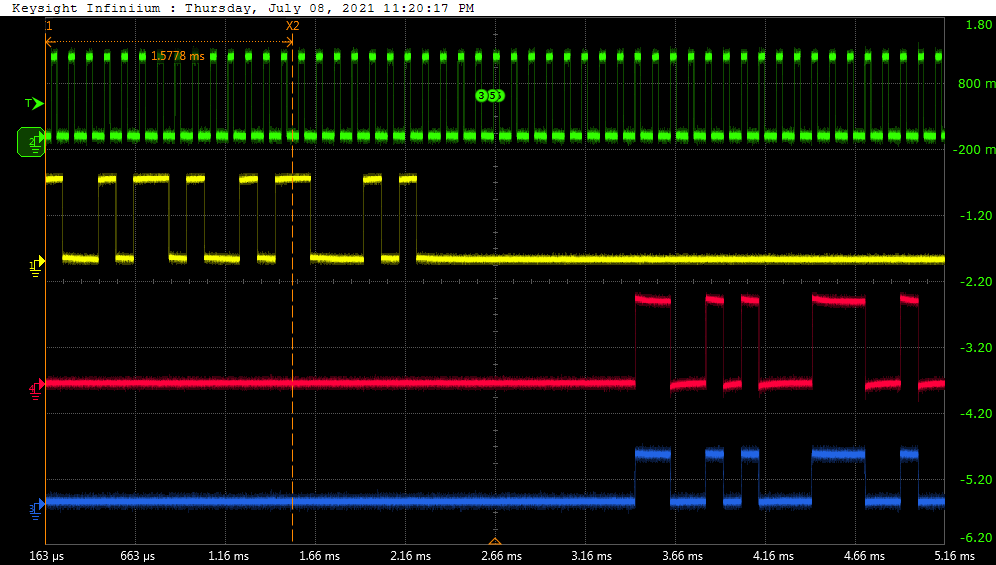
\includegraphics[width=0.95 \textwidth]{IMG/probe/09-08-2021_ch05-read57-baselinedac1.png}
				\caption{\centering{\tiny ch07-read57}}
			\end{figure}
			\begin{figure}
				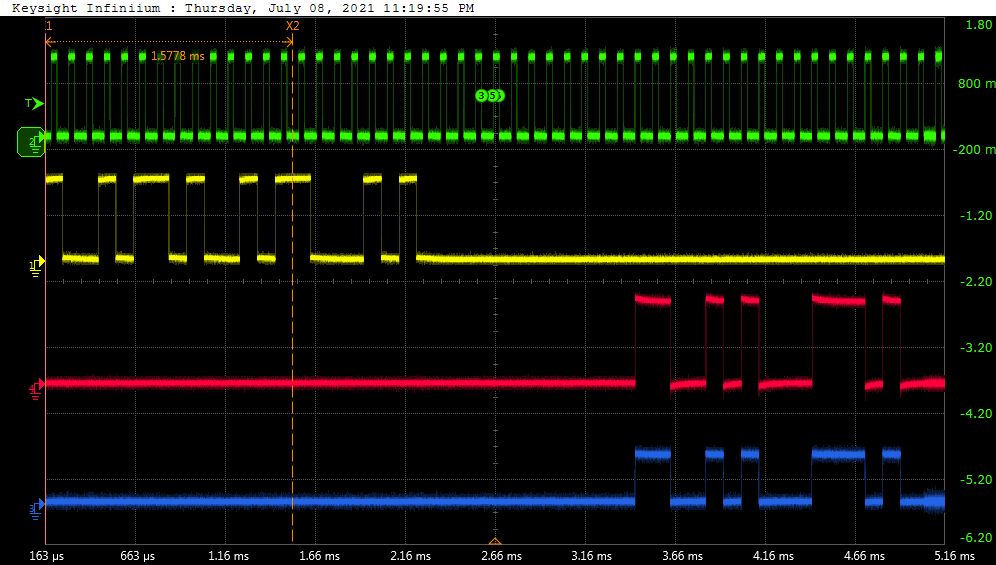
\includegraphics[width=0.95 \textwidth]{IMG/probe/09-08-2021_ch05-read58-baselinedac1.png}
				\caption{\centering{\tiny ch07-read58}}
			\end{figure}	
		\end{center}
		\column{0.3 \textwidth}
		\begin{center}
			\begin{figure}
				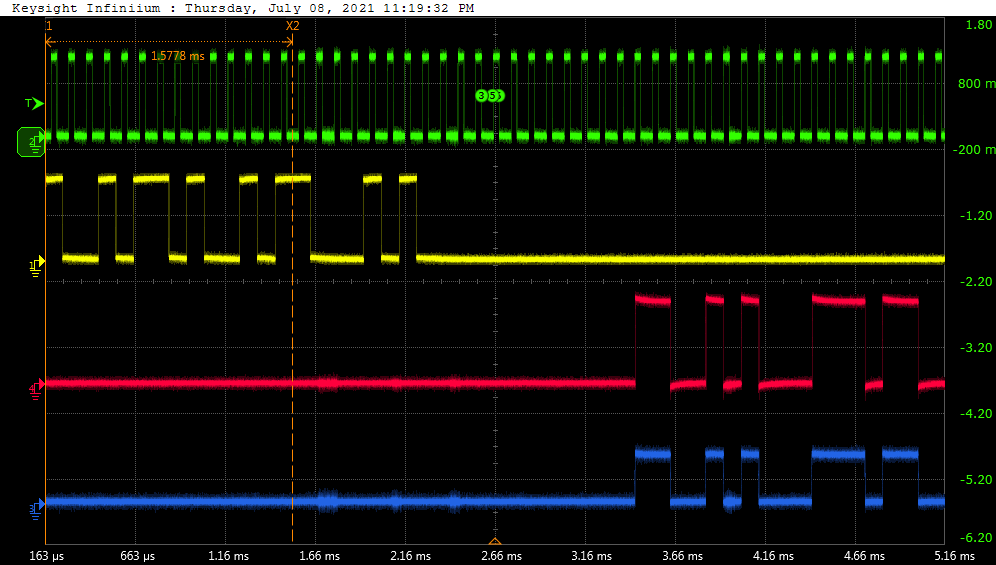
\includegraphics[width=0.95 \textwidth]{IMG/probe/09-08-2021_ch05-read59-baselinedac1.png}
				\caption{\centering{\tiny ch07-read59}}
			\end{figure}
			\begin{figure}
				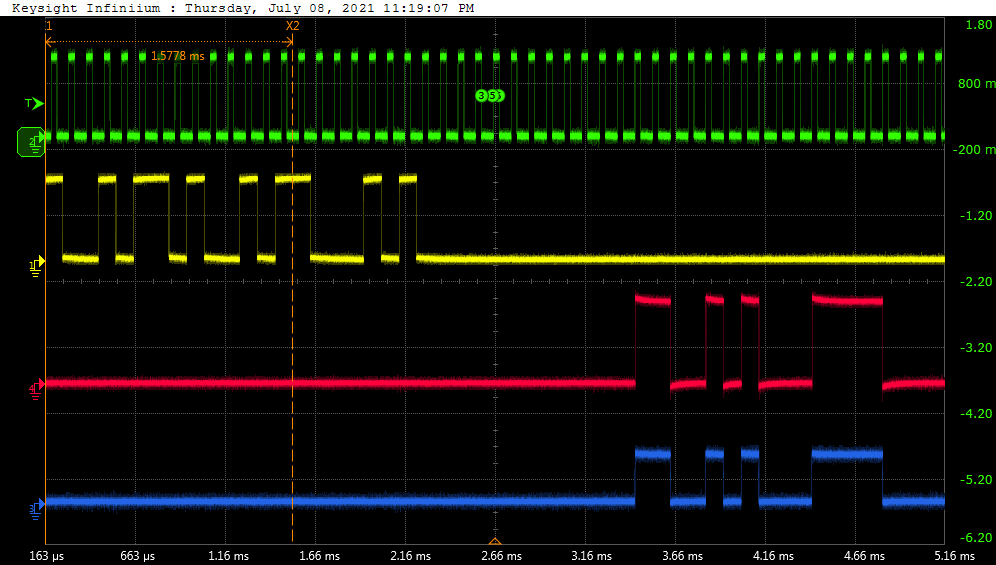
\includegraphics[width=0.95 \textwidth]{IMG/probe/09-08-2021_ch05-read60-baselinedac1.png}
				\caption{\centering{\tiny ch07-read60}}
			\end{figure}	
		\end{center}
	\end{columns}
		\end{frame}
	
	\begin{frame}[noframenumbering]
		\frametitle{CML}
		\begin{columns}
			\column{0.5 \textwidth}
			\begin{center}
				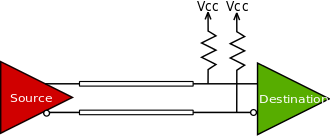
\includegraphics[width=0.95 \textwidth]{IMG/CML_line.png}
			\end{center}
			\column{0.5 \textwidth}
			CML (\textbf{C}urrent \textbf{M}ode \textbf{L}ogic), is a digital design style used both for logic gates and for board-level digital signalling of digital data.
			\begin{itemize}
				\item speeds between 312.5 Mbit/s and 3.125 Gbit/s
				\item DVI and HDMI video links use CML
				\item 50 $\Omega$ termination
			\end{itemize}
		\end{columns}
	\end{frame}

	\begin{frame}[noframenumbering]
		\frametitle{I2C}
		\begin{center}
			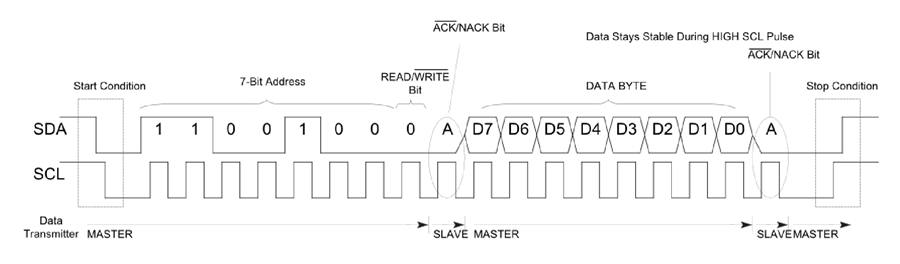
\includegraphics[width=0.8 \textwidth]{IMG/I2C.png}
		\end{center}
		The Inter-Integrated Circuit (I2C) bus is a two wire serial interface originally developed by the Phillips Corporation for use in consumer products. It is a bi-directional bus that is easily implemented in any IC process (NMOS, CMOS, bipolar) and allows for simple inter-IC communication. Connections are minimized by using a serial data line (SDA), a serial clock line (SCL) and a common ground to carry all communications.
	\end{frame}

	\begin{frame}[noframenumbering]
		\frametitle{LVDS}
		\begin{columns}
			\column{0.5 \textwidth}
			\begin{center}
				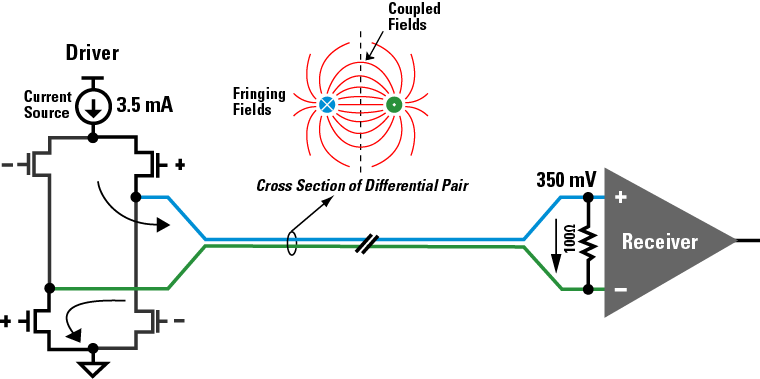
\includegraphics[width=0.95 \textwidth]{IMG/LVDS.png}
			\end{center}
			\column{0.5 \textwidth}
			\begin{itemize}
				\item Low-voltage differential signaling, or LVDS is a technical standard that specifies electrical characteristics of a differential serial signaling standard.
				\item The transmitter injects a constant current of 3.5 mA into the wires
				\item 100 $\Omega$ termination
			\end{itemize}
		\end{columns}
	\end{frame}

	%\begin{frame}[noframenumbering]
	%	\frametitle{Constraints}
	%	\begin{columns}
	%		\column{0.5 \textwidth}
	%		\column{0.5 \textwidth}
	%		\begin{itemize}
	%			\item
	%		\end{itemize}
	%	\end{columns}
	%\end{frame}

	\begin{frame}[noframenumbering]
		\frametitle{UDP}
		\begin{columns}
			\column{0.5 \textwidth}
				\begin{center}
					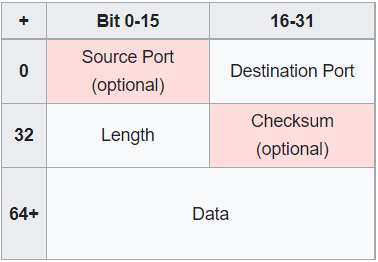
\includegraphics[width=0.95 \textwidth]{IMG/UDP.png}
				\end{center}
			\column{0.5 \textwidth}
			\begin{itemize}
				\item \textbf{UDP}= \textbf{U}ser \textbf{D}atagram \textbf{P}rotocol is one of the core members of the Internet protocol suite. With UDP, computer applications can send messages, in this case referred to as datagrams.
				\item UDP uses a simple connectionless communication model. 
				\item UDP is suitable for purposes where error checking and correction are either not necessary or are performed in the application.
			\end{itemize}
		\end{columns}
	\end{frame}

	\begin{frame}[noframenumbering]
	\frametitle{Reading Baseline DACs $\rightarrow$ code}
	\begin{itemize}
		\item \textbf{reading} procedure for 1 dac consist of \textbf{2 processes}=
		\begin{itemize}
			\item \textbf{16}bit shift register
			\item sequence detector 
		\end{itemize}
	\end{itemize}
	\begin{center}
		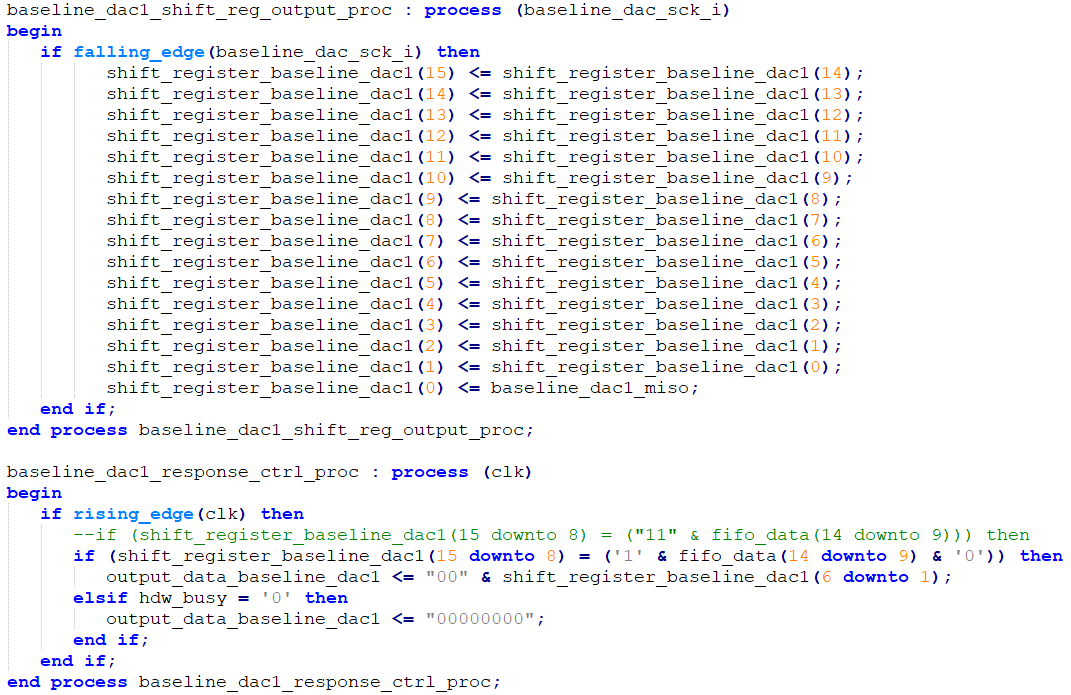
\includegraphics[width=0.6 \textwidth]{IMG/FSM_Read_States.png}
	\end{center}
	\end{frame}

		\begin{frame}[noframenumbering]
	\frametitle{VHDL}
	{\LARGE
		\begin{itemize}
			\item \textbf{VHDL}: \textbf{V}HSIC \textbf{H}ardware \textbf{D}escription \textbf{L}anguage 
			\begin{itemize}
				\item \textbf{VHSIC}: \textbf{V}ery \textbf{H}igh \textbf{S}peed \textbf{I}ntegrated \textbf{C}ircuits
				\item Is a hardware description language (\textbf{HDL}) that can model the behavior and structure of digital systems at multiple levels of abstraction
				\item Since \textbf{1987}, VHDL has been standardized by the Institute of Electrical and Electronics Engineers (\textbf{IEEE})
				\item In February 2008, Accellera approved \textbf{VHDL 4.0}, also informally known as VHDL 2008
				\item {\color{orange} VHDL is not a programming language!}
			\end{itemize}
		\end{itemize}
	}
\end{frame}
	
	\begin{frame}[noframenumbering]
		\frametitle{FPGA structure}
		\begin{itemize}
			\item \textbf{PSM}: \textbf{P}rogrammable \textbf{S}witch \textbf{M}atrix = Whenever a vertical and a horizontal channel intersect, there is a switch box. When a wire enters a switch box there are programmable switches that allow it to connect to other wires in adjacent channel segments
			\item \textbf{IOB}: \textbf{I}/\textbf{O} \textbf{B}lock = collection or grouping of basic elements that implement the input and output functions of an FPGA device
			\item \textbf{CLB}: \textbf{C}onfigurable \textbf{L}ogic \textbf{B}lock = A typical cell consists of a 4-input LUT, a Full adder (FA) and a D-type flip-flop
		\end{itemize}
	\end{frame}
	
\end{document}